\documentclass[a4paper,12pt]{article} % добавить leqno в [] для нумерации слева
\usepackage[a4paper,top=1.3cm,bottom=2cm,left=1.5cm,right=1.5cm,marginparwidth=0.75cm]{geometry}
%%% Работа с русским языком
\usepackage{cmap}					% поиск в PDF
\usepackage{mathtext} 				% русские буквы в фомулах
\usepackage[T2A]{fontenc}			% кодировка
\usepackage[utf8]{inputenc}			% кодировка исходного текста
\usepackage[english,russian]{babel}	% локализация и переносы

\usepackage{graphicx}

\usepackage{wrapfig}
\usepackage{tabularx}

\usepackage{hyperref}
\usepackage[rgb]{xcolor}
\hypersetup{
colorlinks=true,urlcolor=blue
}
\usepackage{multirow}
\usepackage{hhline}


%%% Дополнительная работа с математикой
\usepackage{amsmath,amsfonts,amssymb,amsthm,mathtools} % AMS
\usepackage{icomma} % "Умная" запятая: $0,2$ --- число, $0, 2$ --- перечисление

%% Номера формул
\mathtoolsset{showonlyrefs=true} % Показывать номера только у тех формул, на которые есть \eqref{} в тексте.

%% Шрифты
\usepackage{euscript}	 % Шрифт Евклид
\usepackage{mathrsfs} % Красивый матшрифт

%% Свои команды
\DeclareMathOperator{\sgn}{\mathop{sgn}}

%% Перенос знаков в формулах (по Львовскому)
\newcommand*{\hm}[1]{#1\nobreak\discretionary{}
{\hbox{$\mathsurround=0pt #1$}}{}}

\begin{document}

\newenvironment{lines}[1][\textwidth] % по умолчанию линейки на всю ширину текста
{
\newcolumntype{E}{>{}p{#1}<{\hrulefill}} % в конце нашего столбца будет приписываться \hrulefill
\begin{flushright} % автоматически вставим flushright
\begin{tabular}[h]{E} % и tabular нужного формата
}
{\end{tabular}\end{flushright}
}
	
	\begin{titlepage}
	\begin{center}
		{\large МОСКОВСКИЙ ФИЗИКО-ТЕХНИЧЕСКИЙ ИНСТИТУТ (НАЦИОНАЛЬНЫЙ ИССЛЕДОВАТЕЛЬСКИЙ УНИВЕРСИТЕТ)}
	\end{center}
	\begin{center}
		{\large Физтех-школа электроники, фотоники и молекулярной физики}
	\end{center}
	
	
	\vspace{4.5cm}
	{\huge
		\begin{center}
			{Лабораторная работа 5.5.5}\\
			 Компьютерная сцинтилляционная $\gamma$-спектрометрия
		\end{center}
	}
	\vspace{2cm}
	\begin{flushright}
		{\LARGE Салтыкова Дарья \\
			\vspace{0.5cm}
			Б04-105}
	\end{flushright}
	
	\vspace{0.5cm}
	
	\begin{lines}[.5
	\textwidth]
  {\LARGE Допуск} \rule{6.5cm}{0.25pt} \vspace{0.5cm}\\
 {\LARGE Выполнение} \rule{3cm}{0.25pt}\vspace{0.5cm} \\ {\LARGE Сдача} \rule{3cm}{0.25pt} \\ % \rule сделает линейку указанной длины и толщины
\end{lines}
	\vspace{6cm}
	\begin{center}
		Долгопрудный 2023
	\end{center}
\end{titlepage}

\section{Цель работы}
Снять и исследовать спектры излучения различных источников, характеризовать различные пики в спектрах радиоактивных веществ.

\medskip

\section{В работе используются:}
Cцинтиллятор, ФЭУ, предусилитель импульсов, высоковольтный блок питания для ФЭУ, АЦП, компьютер.

\medskip

\section{Теоретические положения}
\noindent \textbf{Фотоэффект} - это процесс взаимодействия гамма-кванта с электроном, связанным с атомом, при котором электрону передается вся энергия гамма-кванта. При этом электрону сообщается кинетическая энергия $T_e=E_\gamma-I_i$, где $E_\gamma$ -- энергия гамма-кванта, $I_i$ -- потенциал ионизации $i$-той оболочки атома. Фотоэффект особенно существенен для тяжелых веществ, где он идет с заметной вероятностью даже при высоких энергиях гамма-квантов. В легких веществах фотоэффект становится заметен лишь при относительно небольших энергиях гамма-квантов. 

\medskip 

\noindent \textbf{Эффект Комптона} - это упругое рассеяние фотона на свободном электроне, сопровождающееся изменением длины волны фотона. Максимальная энергия образующихся комптоновских электронов соответствует рассеянию гамма-квантов на $180^\circ$ и равна

\begin{equation}
E_{\max}=\frac{\eta\omega}{1+\frac{mc^2}{2\eta\omega}}.
\end{equation}

\medskip

\noindent \textbf{Процесс образования электрон-позитронных пар.}
При достаточно высокой энергии гамма-кванта наряду с фотоэффектом и эффектом Комптона может происходить третий вид взаимодействия гамма-квантов с веществом -- образование электрон-позитронных пар. Процесс образования пар не может происходить в пустоте, так как в этом случае не выполняются законы сохранения энергии и импульса. В присутствии ядра или электрона процесс образования пары гамма-квантов возможен, так как можно распределить энергию и импульс гамма-кванта между тремя частицами без противоречия с законами сохранения. При этом если процесс образования пары идет в кулоновском поле ядра или протона, то энергия образующегося ядра отдачи оказывается весьма малой, так что пороговая энергия гамма-кванта $E_0$, необходимая для образования пары, практически совпадает с удвоенной энергией покоя электрона $E_0\cong 2mc^2=1.022$ МэВ.


\medskip

\noindent Появившийся в результате процесса образования пар электрон свою энергию на ионизацию среды. Таким образом, вся энергия электрона остается в детекторе. Позитрон будет двигаться до тех пор, пока практически не остановится, а затем аннигилирует с электроном среды, в результате чего появятся два гамма-кванта. Т.е., кинетическая энергия позитрона также останется в детекторе. Далее возможны три варианта развития событий:

\medskip

\begin{enumerate}
\item оба родившихся гамма-кванта не вылетают из детектора, и тогда вся энергия первичного гамма-кванта останется в детекторе, а в спектре появится пик с $E=E_{\gamma}$;
\item один из родившихся гамма-квантов покидает детектор, и в спектре появляется пик, соответствующий энергии $E=E_{\gamma}-E_0$, где $E_0=mc^2=511$ кэВ;
\item оба родившихся гамма-кванта покидают детектор, и в спектре появляется пик, соотвествующий энергии $E=E_{\gamma}-2E_0$, где $2E_0=2mc^2=1022$ кэВ.
\end{enumerate}

\medskip

\noindent Таким образом, любой спектр, получаемый с помощью гамма-спектрометра, описывается несколькими компонентами, каждая из которых связана с определенным физическим процессом. Как описано выше, основными физическими процессами взаимодействия гамма-квантов с веществом является фотоэффект, эффект Комптона и образование электрон-позитронных пар, и каждый из них вносит свой вклад в образование спектра. Помимо этих процессов, добавляется \textit{экспонента}, связанная с наличием фона, \textit{пик характеристического излучения}, возникающий при взаимодействии гамма-квантов с окружающим веществом, а также \textit{пик обратного рассеяния}, образующийся при энергии квантов $E_{\gamma}\gg mc^2/2$ в результате рассеяния гамма-квантов на большие углы на материалах  конструктивных элементов детектора и защиты. Положение пика обратного рассеяния определяется по формуле:

\medskip

\begin{equation}
E_{\text{обр}}=\frac{E}{1+2E/mc^2},
\label{eq:Ereverse}
\end{equation}

\medskip

\noindent где $E$ -- энергия фотопика.

\medskip

\noindent \paragraph{Энергетическое разрешение спектрометра.} Даже при поглощении частиц с одинаковой энергией амплитуда импульса на выходе фотоприёмника сцинтилляционного детектора меняется от события к событию. Это связано:

\medskip

\begin{enumerate}
\item со статистическим характером процессов сбора фотонов на фотоприёмнике и последующего усиления,
\item с различной вероятностью доставки фотона к фотоприемнику из разных точек сцинтиллятора,
\item с разбросом высвечиваемого числа фотонов
\end{enumerate}

\medskip

\noindent В результате в набранном спектре линия (которая для идеального детектора представляла бы дельта-функцию) оказывается размытой, её часто описывают гауссианом.\par
Энергетическим разрешением спектрометра называется величина

\medskip

\begin{equation}
R_i=\frac{\Delta E_i}{E_i},
\end{equation}

\medskip

\noindent где $\Delta E_i$ -- ширина пика полного поглощения, измеренная на половине высоты, $E_i$ -- энергия регистрируемого $\gamma$-излучения. Значение $E_i$ пропорционально среднему числу фотонов $\overline{n_i}$ на выходе ФЭУ, т.е.:

\medskip

\begin{equation}
E_i=\alpha\overline{n_i}.
\label{eq:4}
\end{equation}

\medskip

\noindent Полуширина пика полного поглощения $\Delta E_i$ пропорциональна среднеквадратичной флуктуации $\overline{\Delta n_i}$. Т.к. $n_i$ является дискретной случайной величиной, которая распределена по закону Пуассона, то $\overline{\Delta n_i}=\sqrt{\overline{n_i}}$ и поэтому

\medskip

\begin{equation}
\Delta E_i=\alpha\overline{\Delta n_i}=\alpha\sqrt{\overline{n_i}}.
\label{eq:5}
\end{equation}

\medskip


\noindent Из (\ref{eq:4}), (\ref{eq:5}) получаем, что
\begin{equation}
R_i=\frac{\Delta E_i}{E_i}=\frac{\text{const}}{\sqrt{E_i}}.
\label{eq:6}
\end{equation}

\medskip

\noindent Поскольку энергетическое разрешение зависит от энергии, его следует указывать для конкретной энергии. Чаще всего разрешение указывают для энергии гамма-линии $^{137}\text{Cs}$ (661.7 кэВ).

\newpage

\section{Ход работы}

\noindent 1. Проведем измерения гамма-спектров для $^{137}Cs, ^{22}Na, ^{60}Co, ^{241}Am, ^{152}Eu,$ а также измерение фона. Вычтем фон и определим номера каналов, отвечающие центрам пиков полного поглощения $^{137}Cs, ^{22}Na, ^{60}Co$, см. Приложение.

\medskip

\noindent  Построим калибровочный график зависимости номера канала от энергии $\gamma$-кванта (Рис. 1).

\medskip


\begin{figure}[h!]
    \centering
    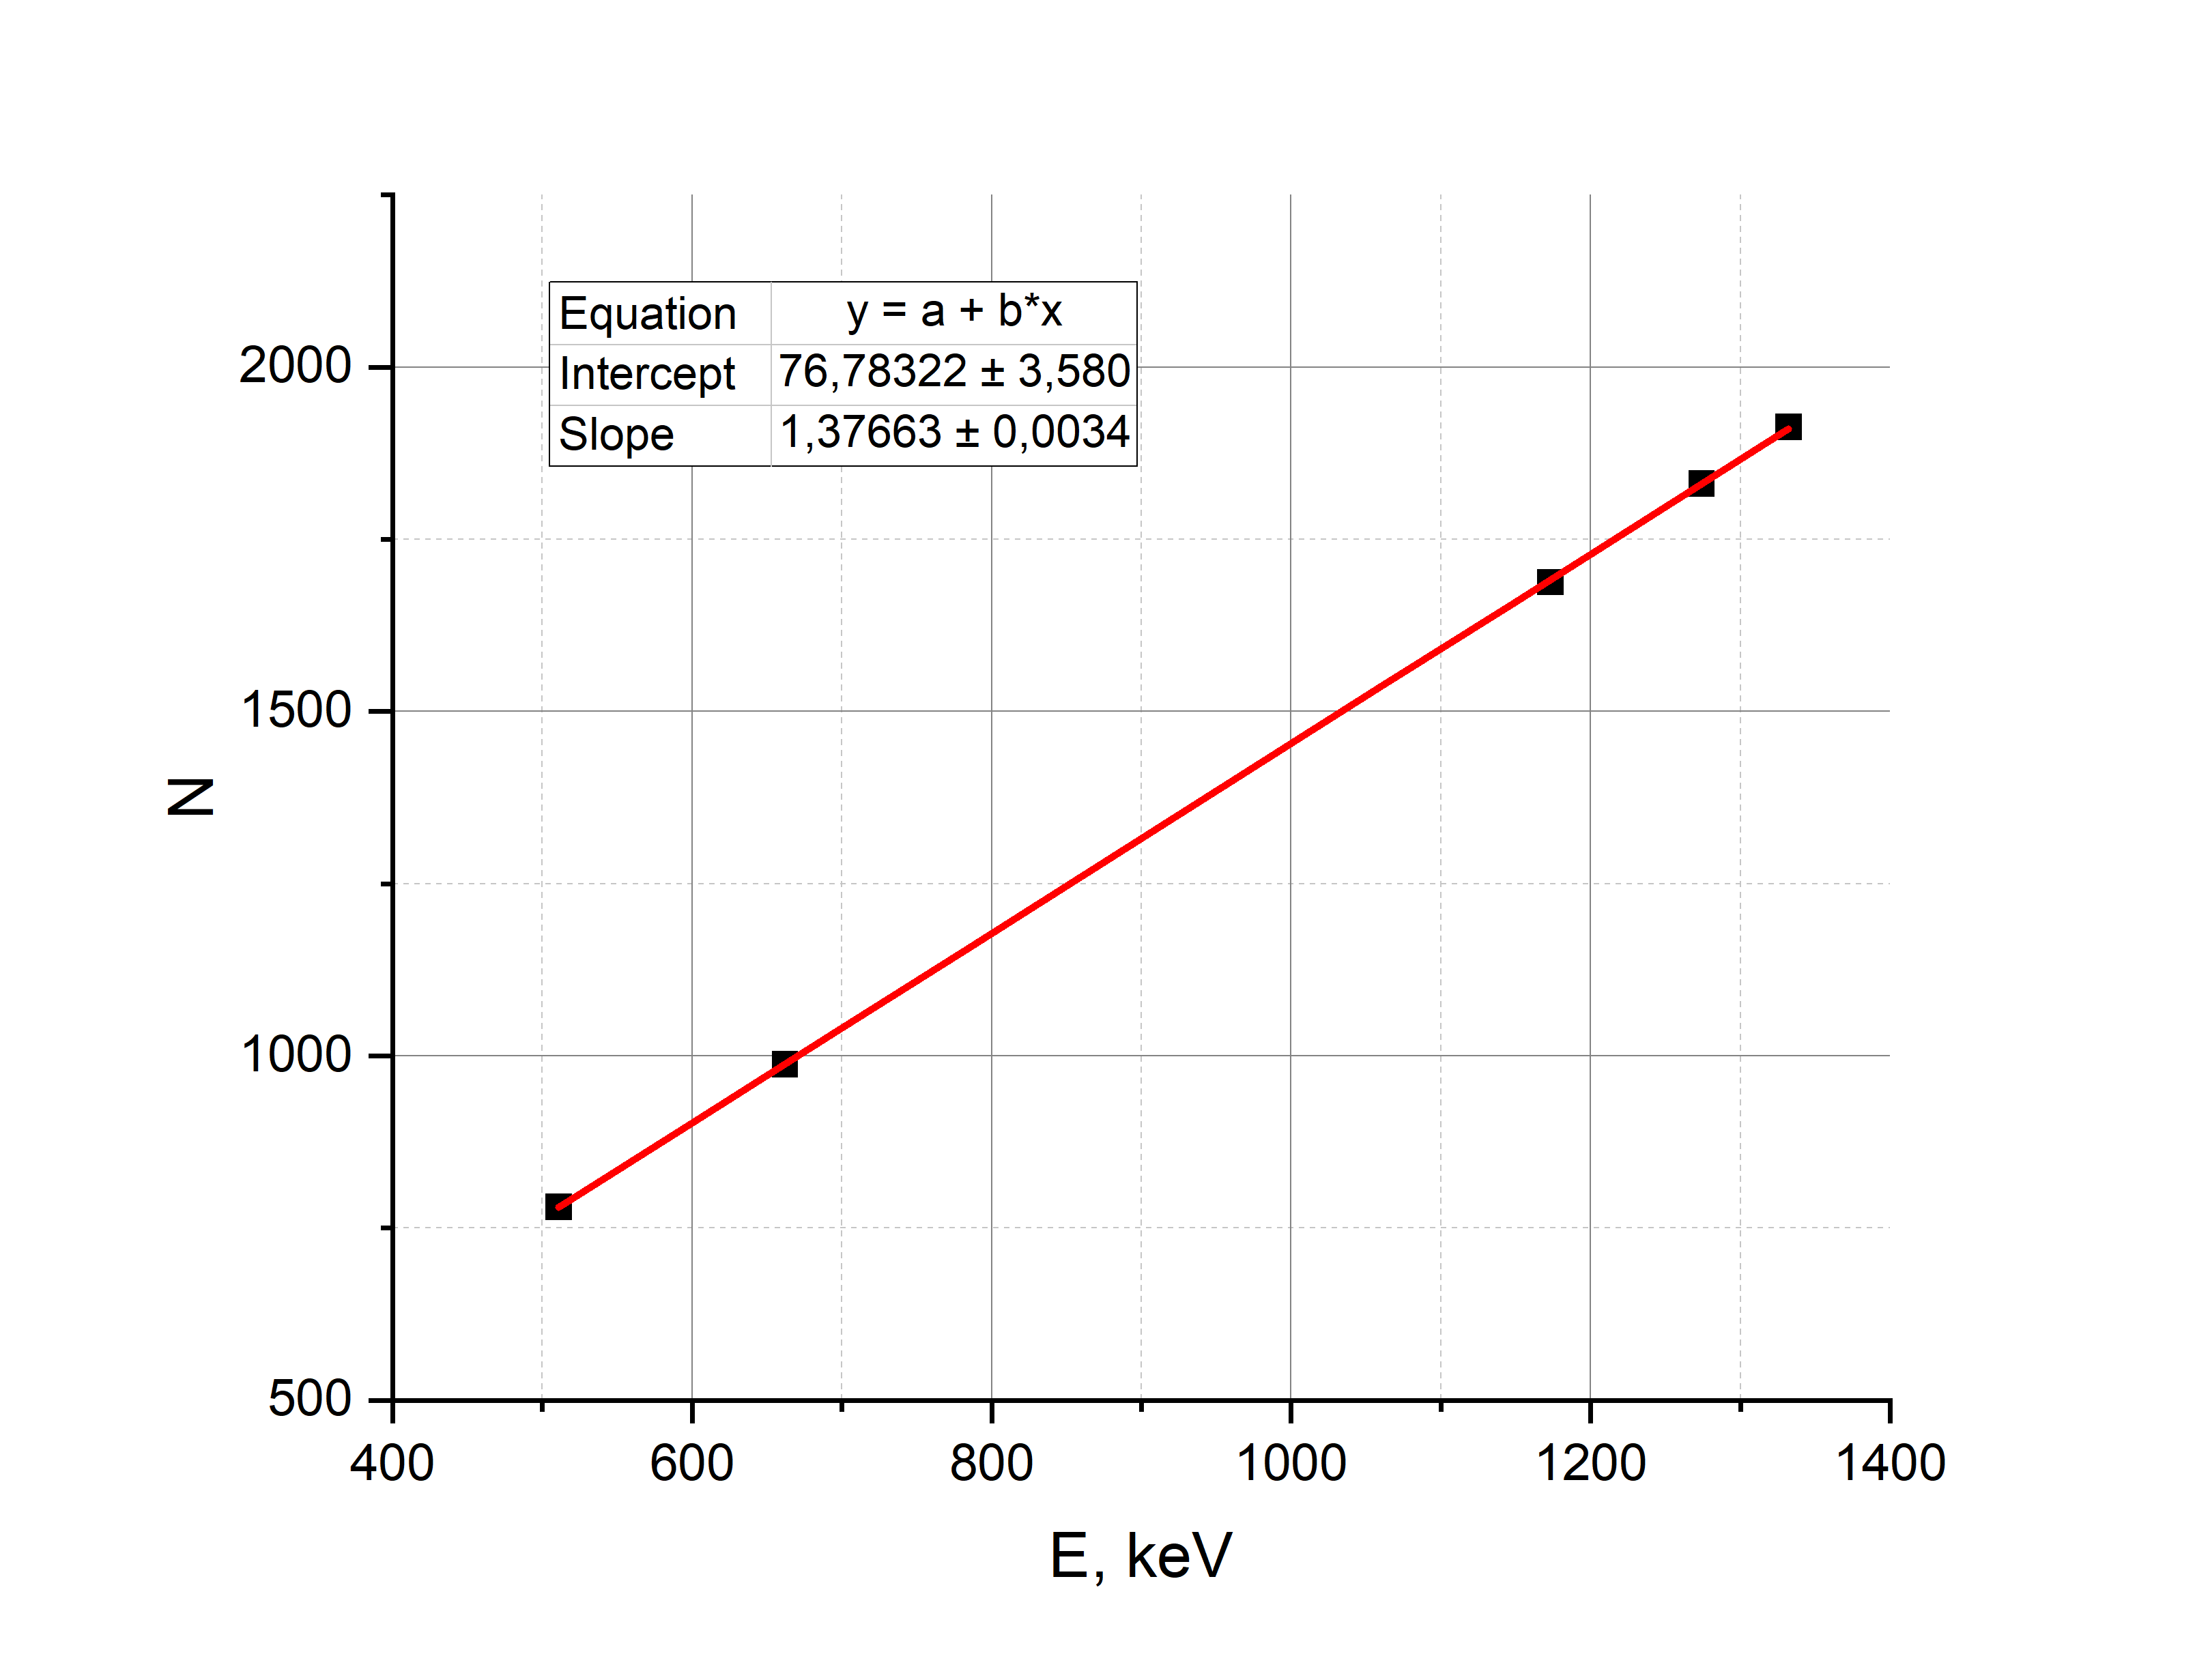
\includegraphics[scale=0.5]{kalibrovka.png}
    \caption{Калибровочный график}
    
\end{figure}


\noindent Используя калибровочный график, определим для всех остальных источников значения энергии пиков полного полного поглощения $E$, их ширины на полувысоте $\Delta E$, и энергетическое разрешение $R$. Результаты сведем в таблицу.

\medskip

\begin{table}[h!]
\begin{tabular}{|l|l|l|l|l|l|l|l|}
\hline
Образец    & N    & $\Delta N$ & $E, \text{ кэВ}$ & $\Delta E, \text{ кэВ}$ & R        & $1/E, \text{ 1/кэВ}$ & $R^2$    \\ \hline
$^{22}Na$  & 781  & 34         & 511,7881         & 24,7093                 & 0,04828  & 0,001954             & 0,002331 \\ \hline
$^{22}Na$  & 1831 & 91         & 1274,869         & 66,1337                 & 0,051875 & 0,000784             & 0,002691 \\ \hline
$^{137}Cs$ & 988  & 77         & 662,2241         & 55,95929                & 0,084502 & 0,00151              & 0,007141 \\ \hline
$^{60}Co$  & 1688 & 120        & 1170,945         & 87,20928                & 0,074478 & 0,000854             & 0,005547 \\ \hline
$^{60}Co$  & 1913 & 196        & 1334,462         & 142,4418                & 0,106741 & 0,000749             & 0,011394 \\ \hline
$^{152}Eu$ & 136  & 21         & 43,03818         & 15,26162                & 0,354607 & 0,023235             & 0,125746 \\ \hline
$^{152}Eu$ & 249  & 33         & 125,1603         & 23,98255                & 0,191615 & 0,00799              & 0,036716 \\ \hline
$^{152}Eu$ & 548  & 16         & 342,4567         & 11,6279                 & 0,033954 & 0,00292              & 0,001153 \\ \hline
$^{241}Am$ & 116  & 18         & 28,5033          & 13,08139                & 0,458943 & 0,035084             & 0,210629 \\ \hline
$^{241}Am$ & 167  & 2          & 65,56725         & 1,453488                & 0,022168 & 0,015252             & 0,000491 \\ \hline
\end{tabular}
\end{table}

\medskip

\begin{table}[h!]
\begin{tabular}{|l|l|l|l|l|}
\hline
Образец    & $E_{\text{теор}}, \text{ кэВ}$ & $E_\text{компт}, \text{ кэВ}$ & $E_\text{расч}, \text{ кэВ}$ & $E_\text{обр}, \text{ кэВ}$ \\ \hline
$^{22}Na$  & 511                            & 325,0149                      & 340                          &                             \\ \hline
$^{22}Na$  & 1274                           & 1086,643                      & 1062                         & 187,6602                    \\ \hline
$^{137}Cs$ & 662                            & 476,9044                      & 477                          & 206,5556                    \\ \hline
$^{60}Co$  & 1173                           & 1016,148                      & 963                          & 232,7184                    \\ \hline
$^{60}Co$  & 1332                           &                               &                              &                             \\ \hline
$^{152}Eu$ & 41,2                           &                               &                              & 43,03818                    \\ \hline
$^{152}Eu$ & 121                            &                               &                              &                             \\ \hline
$^{152}Eu$ & 344                            &                               &                              &                             \\ \hline
$^{241}Am$ & 26,3                           &                               &                              &                             \\ \hline
$^{241}Am$ & 59,6                           &                               &                              &                             \\ \hline
\end{tabular}
\end{table}

\noindent 2. По результатам измерения энергии края комптоновского поглощения построим график, по одной оси которого отложим экспериментальные значения, а по другой расчетные значения этой энергии (Рис. 2).


\begin{figure}[h!]
    \centering
    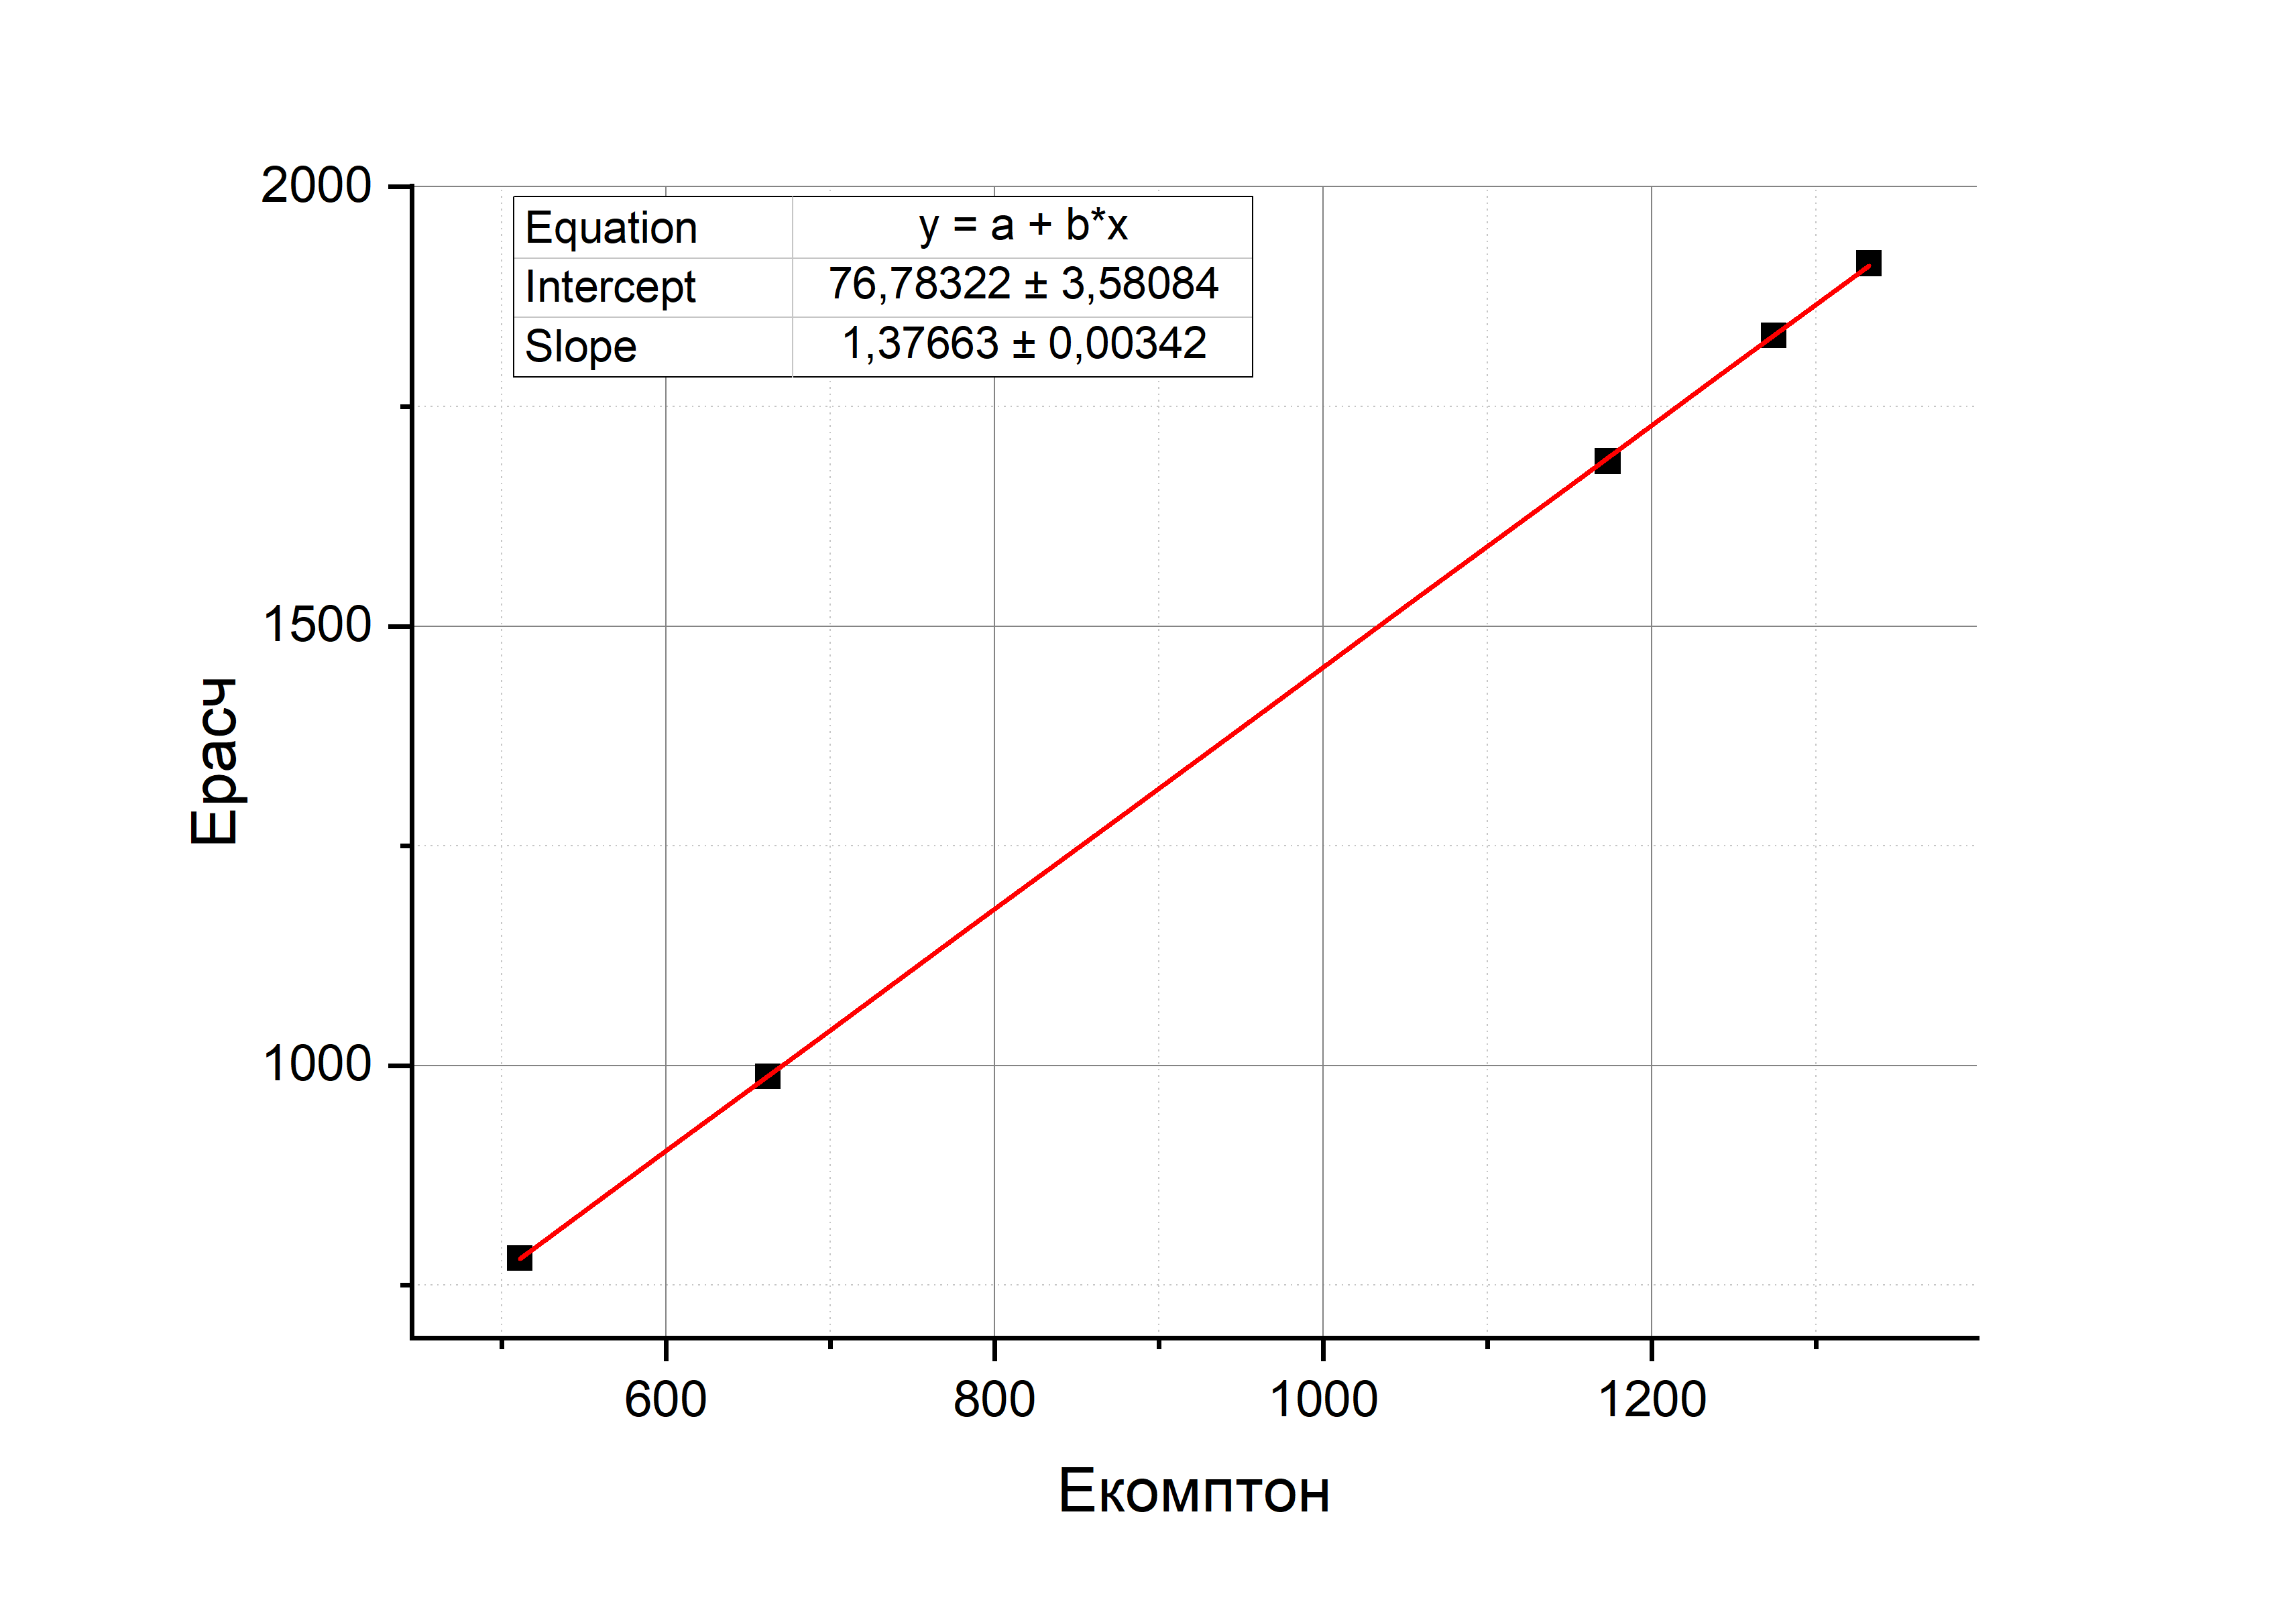
\includegraphics[scale=0.5]{комптон.png}
    \caption{Энергия края комптоновского поглощения: зависимость экспериментальных значений от расчетных}
    
\end{figure}

\medskip


\noindent  Коэффициент при абсциссе близок к единице, а значит экспериментальные значения близки к расчетным.

\medskip

\noindent 3. Построим график $R^2 = f(1/E)$. Значение минимальной энергии для $^{241}Am$ из-за большой погрешности исключим (Рис. 3).


\begin{figure}[h!]
    \centering
    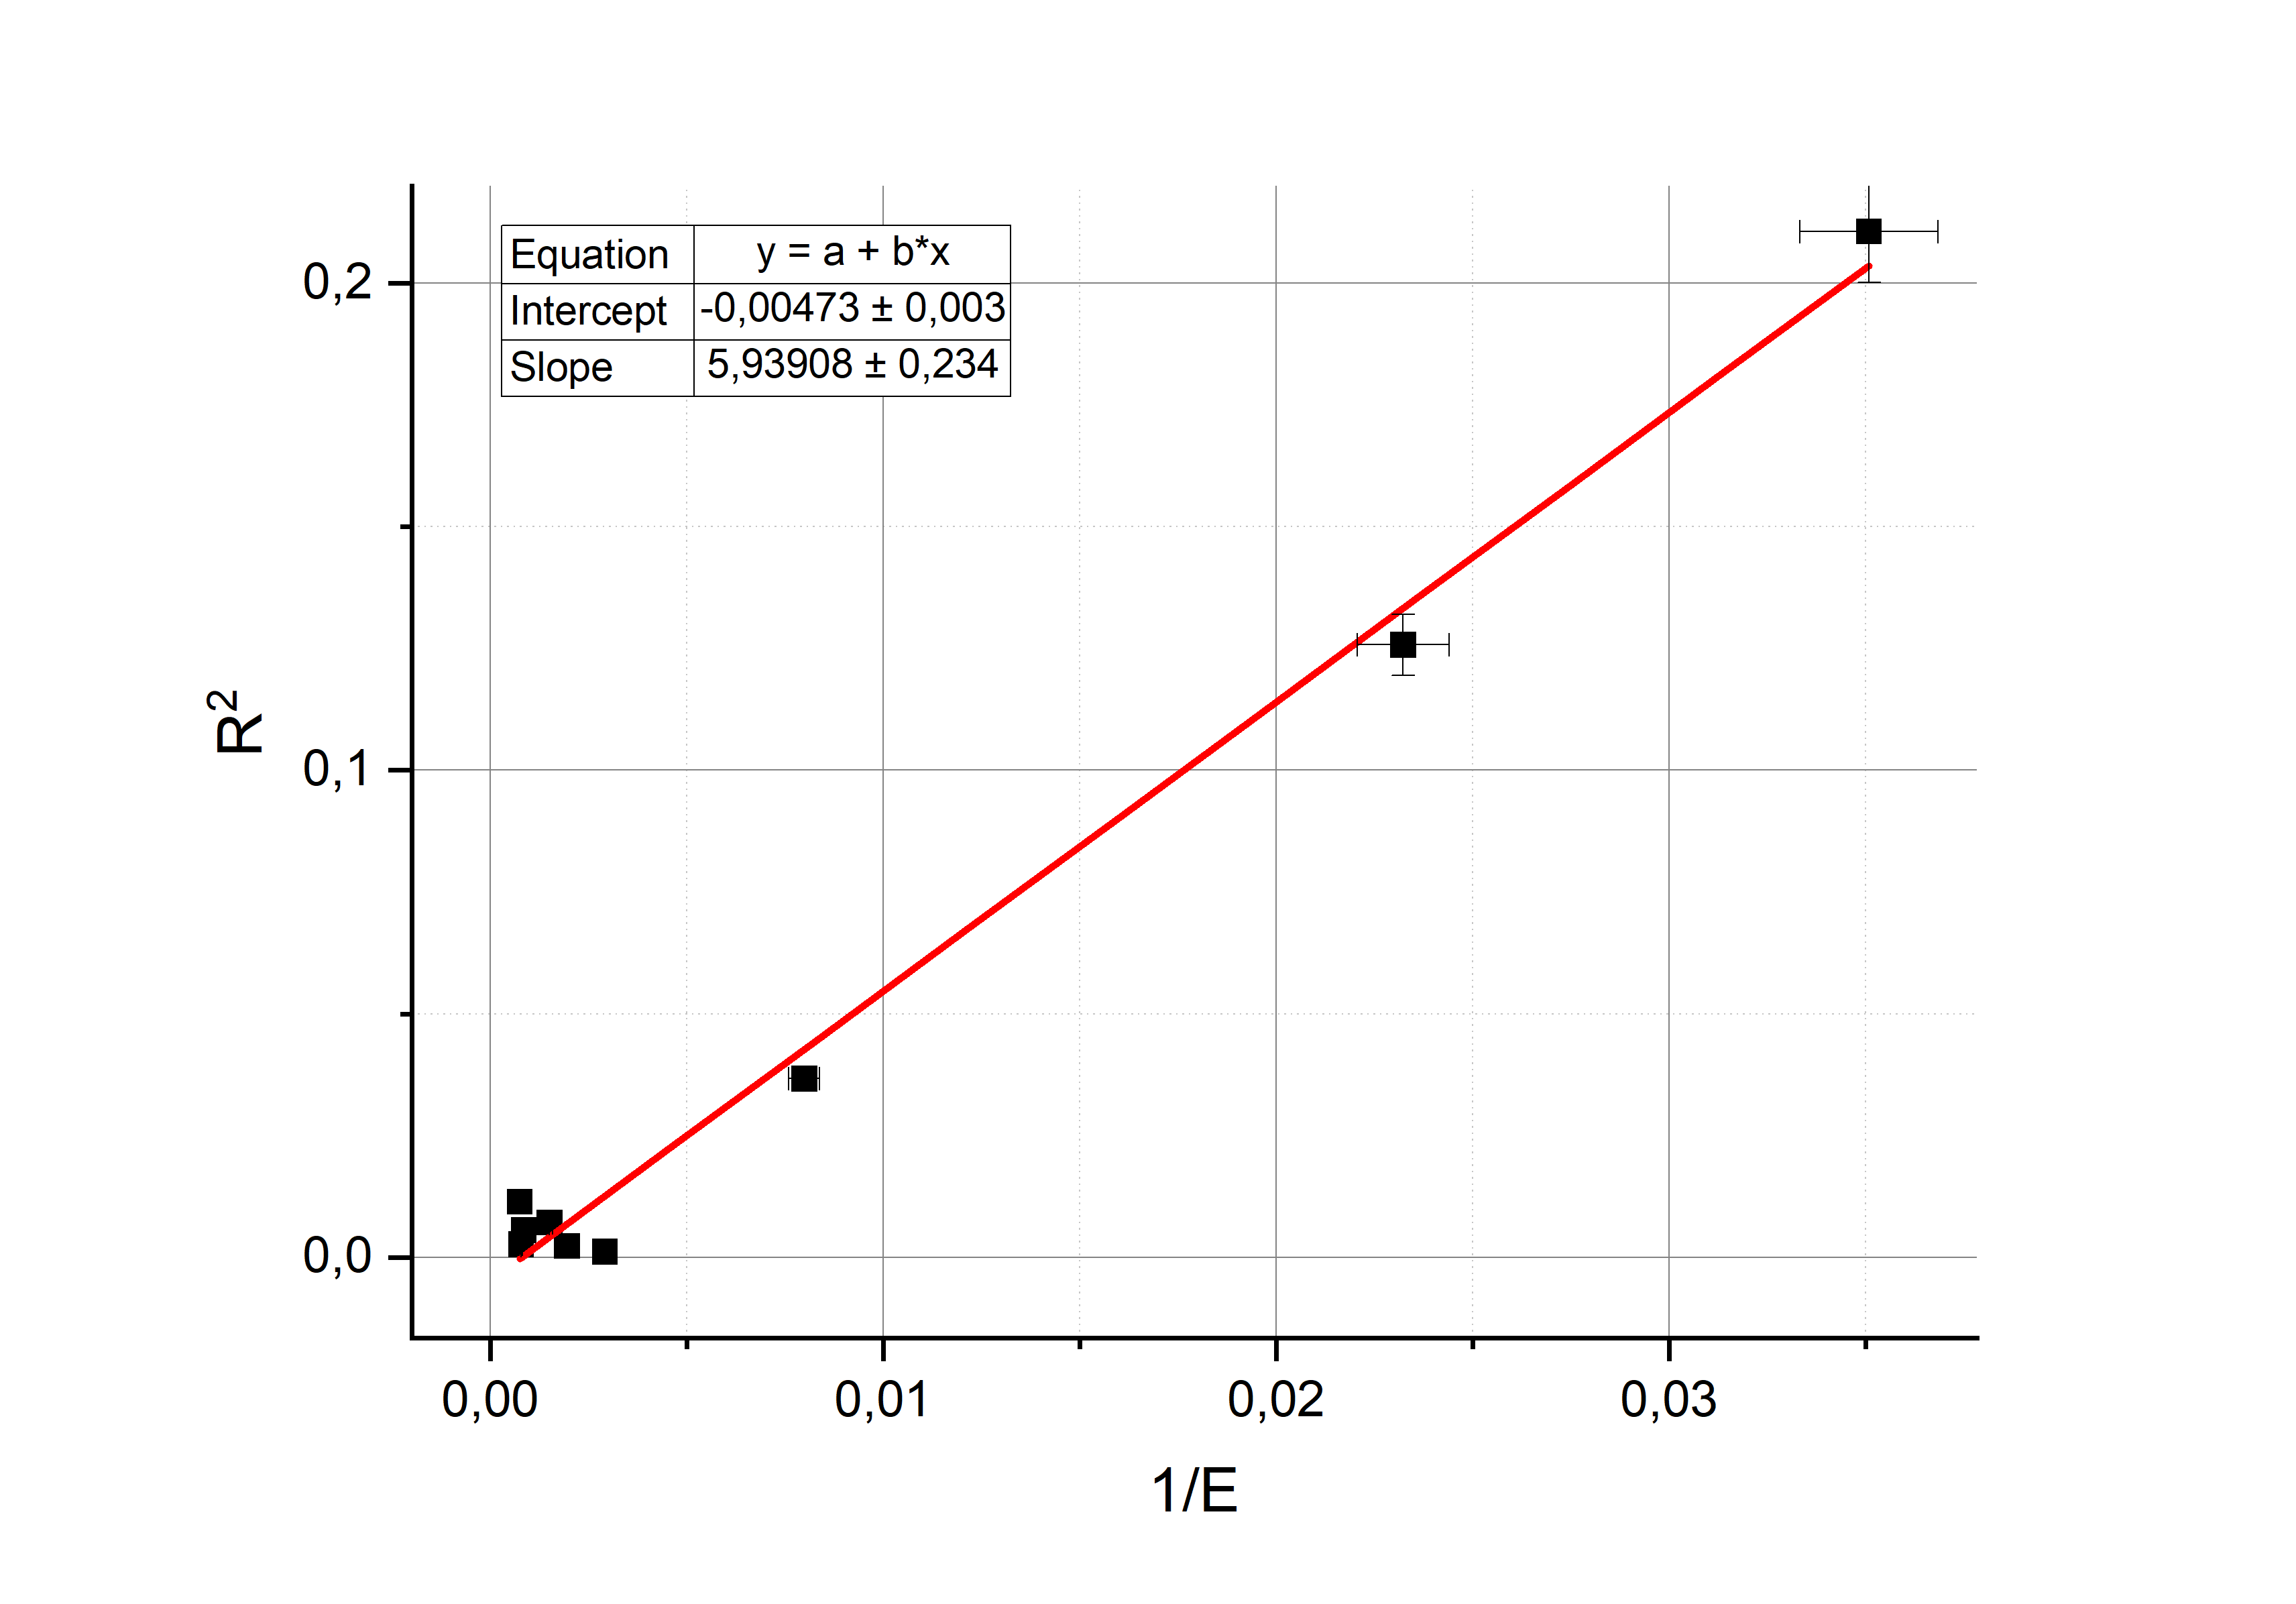
\includegraphics[scale=0.5]{line.png}
    \caption{Зависимость спектрального разрешения прибора от величины, обратной энергии полного поглощения}
    
\end{figure}

\medskip


\noindent 4. Построим график зависимости энергии пика обратного рассеяния от энергии фотопика (Рис. 4).

\begin{figure}[h!]
    \centering
    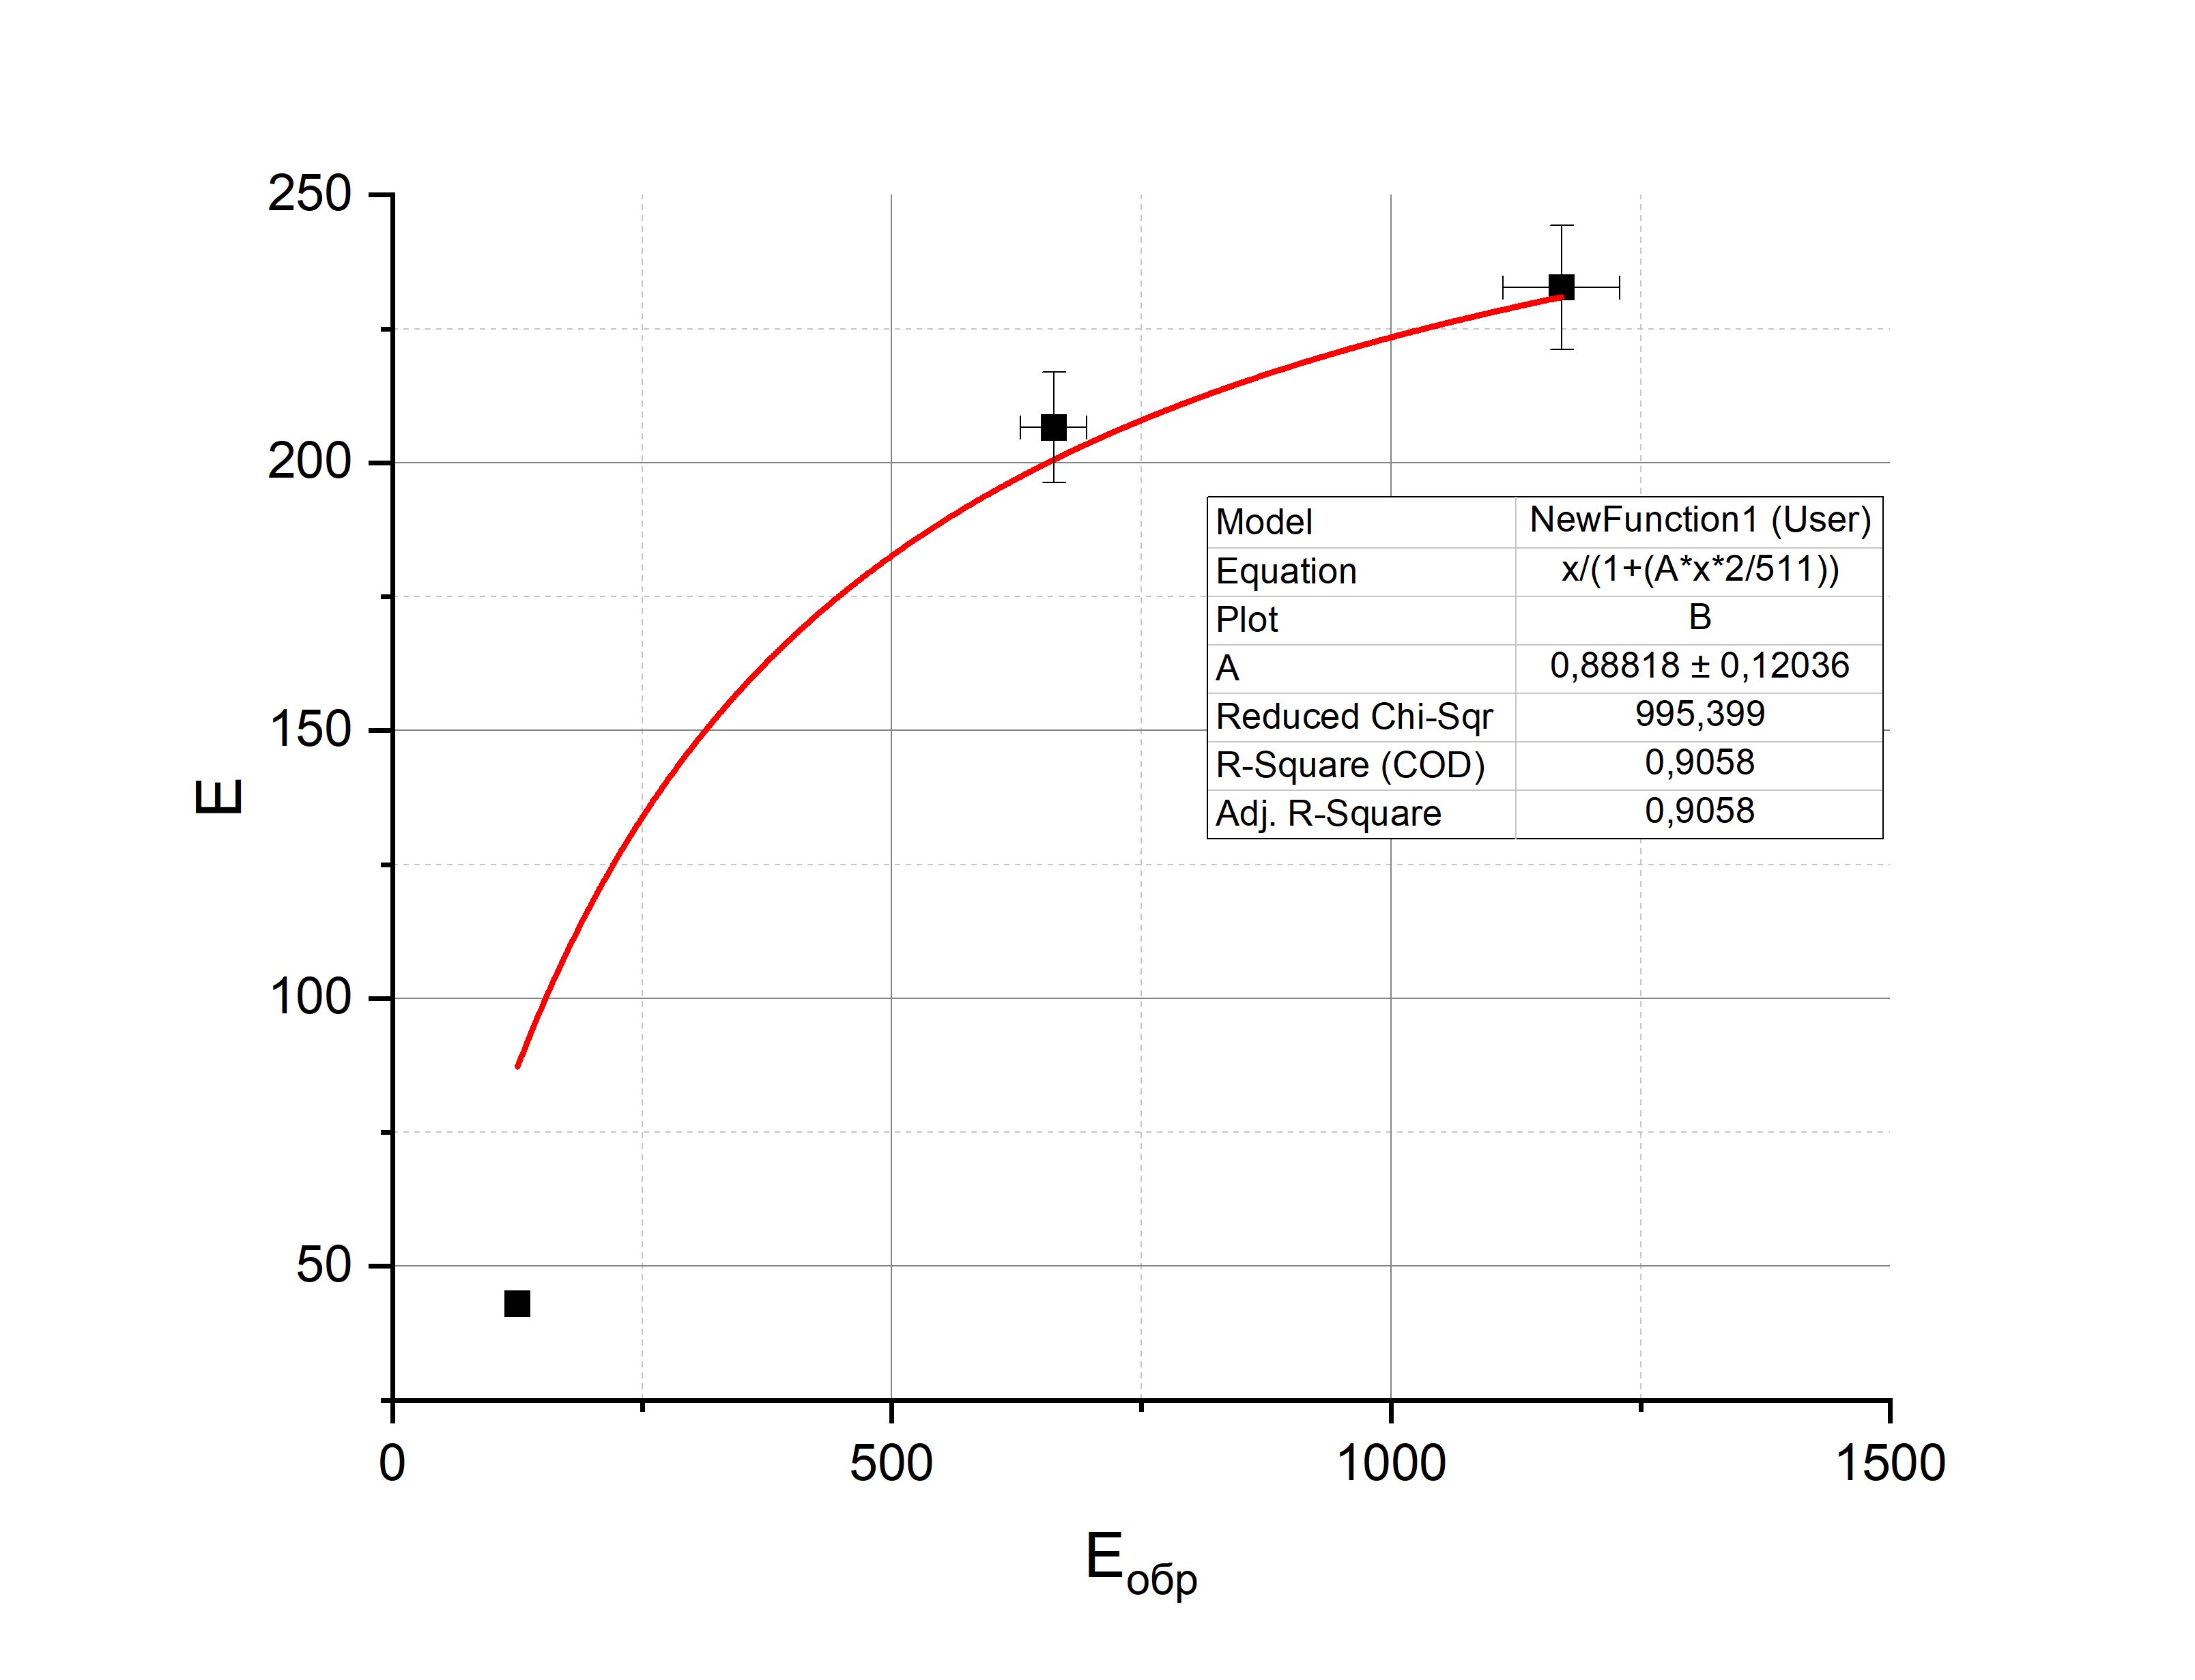
\includegraphics[scale=0.5]{Eobr.png}
    \caption{Зависимость энергии пика обратного рассеяния от энергии фотопика}
    
\end{figure}

\medskip

\noindent 5. Получим на экране осциллографа устойчивое изображение импульсов с выхода ФЭУ. Для лучшего наблюдения импульсов приставим к экрану осциллографа специальный резиновый кожух, предохраняющий от внешней засветки. Форма импульсов на выходе ФЭУ определется выражением:

$$ U(t) = const \cdot e^{-\frac{t}{RC}}(1-e^{-\frac{t}{\tau_0}}),$$

\noindent где $\tau_0$ - время высвечивания сцинтиллятора, RC - постоянная времени (R и C - сопротивление и емкость в анодной цепи ФЭУ). Данное выражение справедливо при $RC >> \tau_0$. По фотографии импульсов оценим величину $\tau_0$ (по переднему фронту импульса) и постоянную времени RC(по заднему фронту импульса):

$$ \tau_0 \approx 2 \text{ мкс}, RC \approx 10 \text{ мкс}.$$

\begin{figure}[h!]
    \centering
    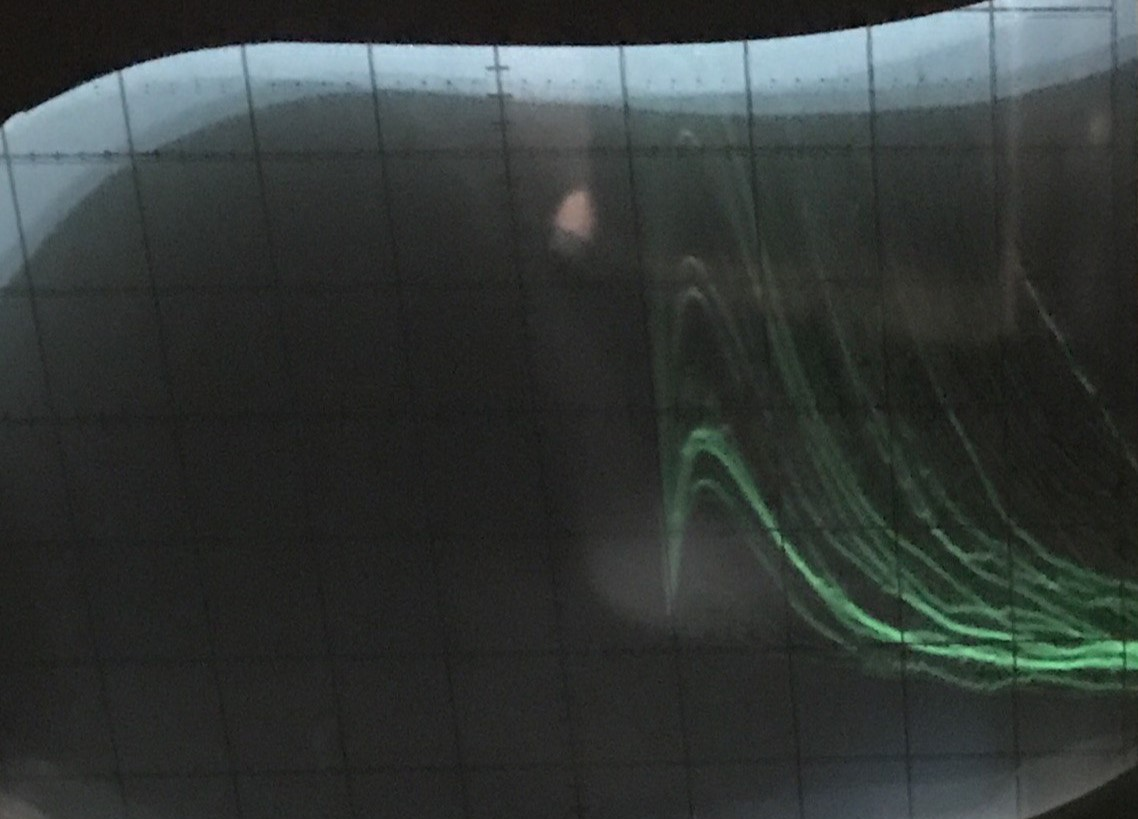
\includegraphics[scale=0.2]{фэу.jpg}
    \caption{Осциллограмма импульсов с выхода ФЭУ}
    
\end{figure}

\section{Вывод}

\noindent В ходе работы были сняты и исследованы спектры образцов $^{137}Cs,  ^{22}Na,  ^{60}Co,  ^{241}Am,  ^{152}Eu$. Были определены пики полного поглощения (фотопики), комптоновские края, пики обратного рассеяния, пик аннигиляции позитронов в спектре натрия (511 кЭв). Полученные экспериментально значения энергий пиков хорошо сходятся с табличными.

\medskip

\noindent Также была проверена линейная зависимость спектрального разрешения прибора от $1/E$, где E - энергия полного поглощения.

\medskip

\noindent По осциллограмме импульсов с выхода ФЭУ определены время высвечивания сцинтиллятора $\tau_0$ и RC - постоянная времени: $ \tau_0 \approx 2 \text{ мкс}, RC \approx 10 \text{ мкс}.$ 

\medskip

\noindent Заметим, что на графиках для цезия и европия в левой части спектра присутствует узкий пик, предположительно соответстсующий характеристическому излучению свинца, служащего защитой спектрометра от внешнего излучения. Энергия этого пика $E_{\text{ свинца}} \approx 40 \text{ кэВ} $.

\newpage

\section{Приложение}

\begin{figure}[h!]
    \centering
    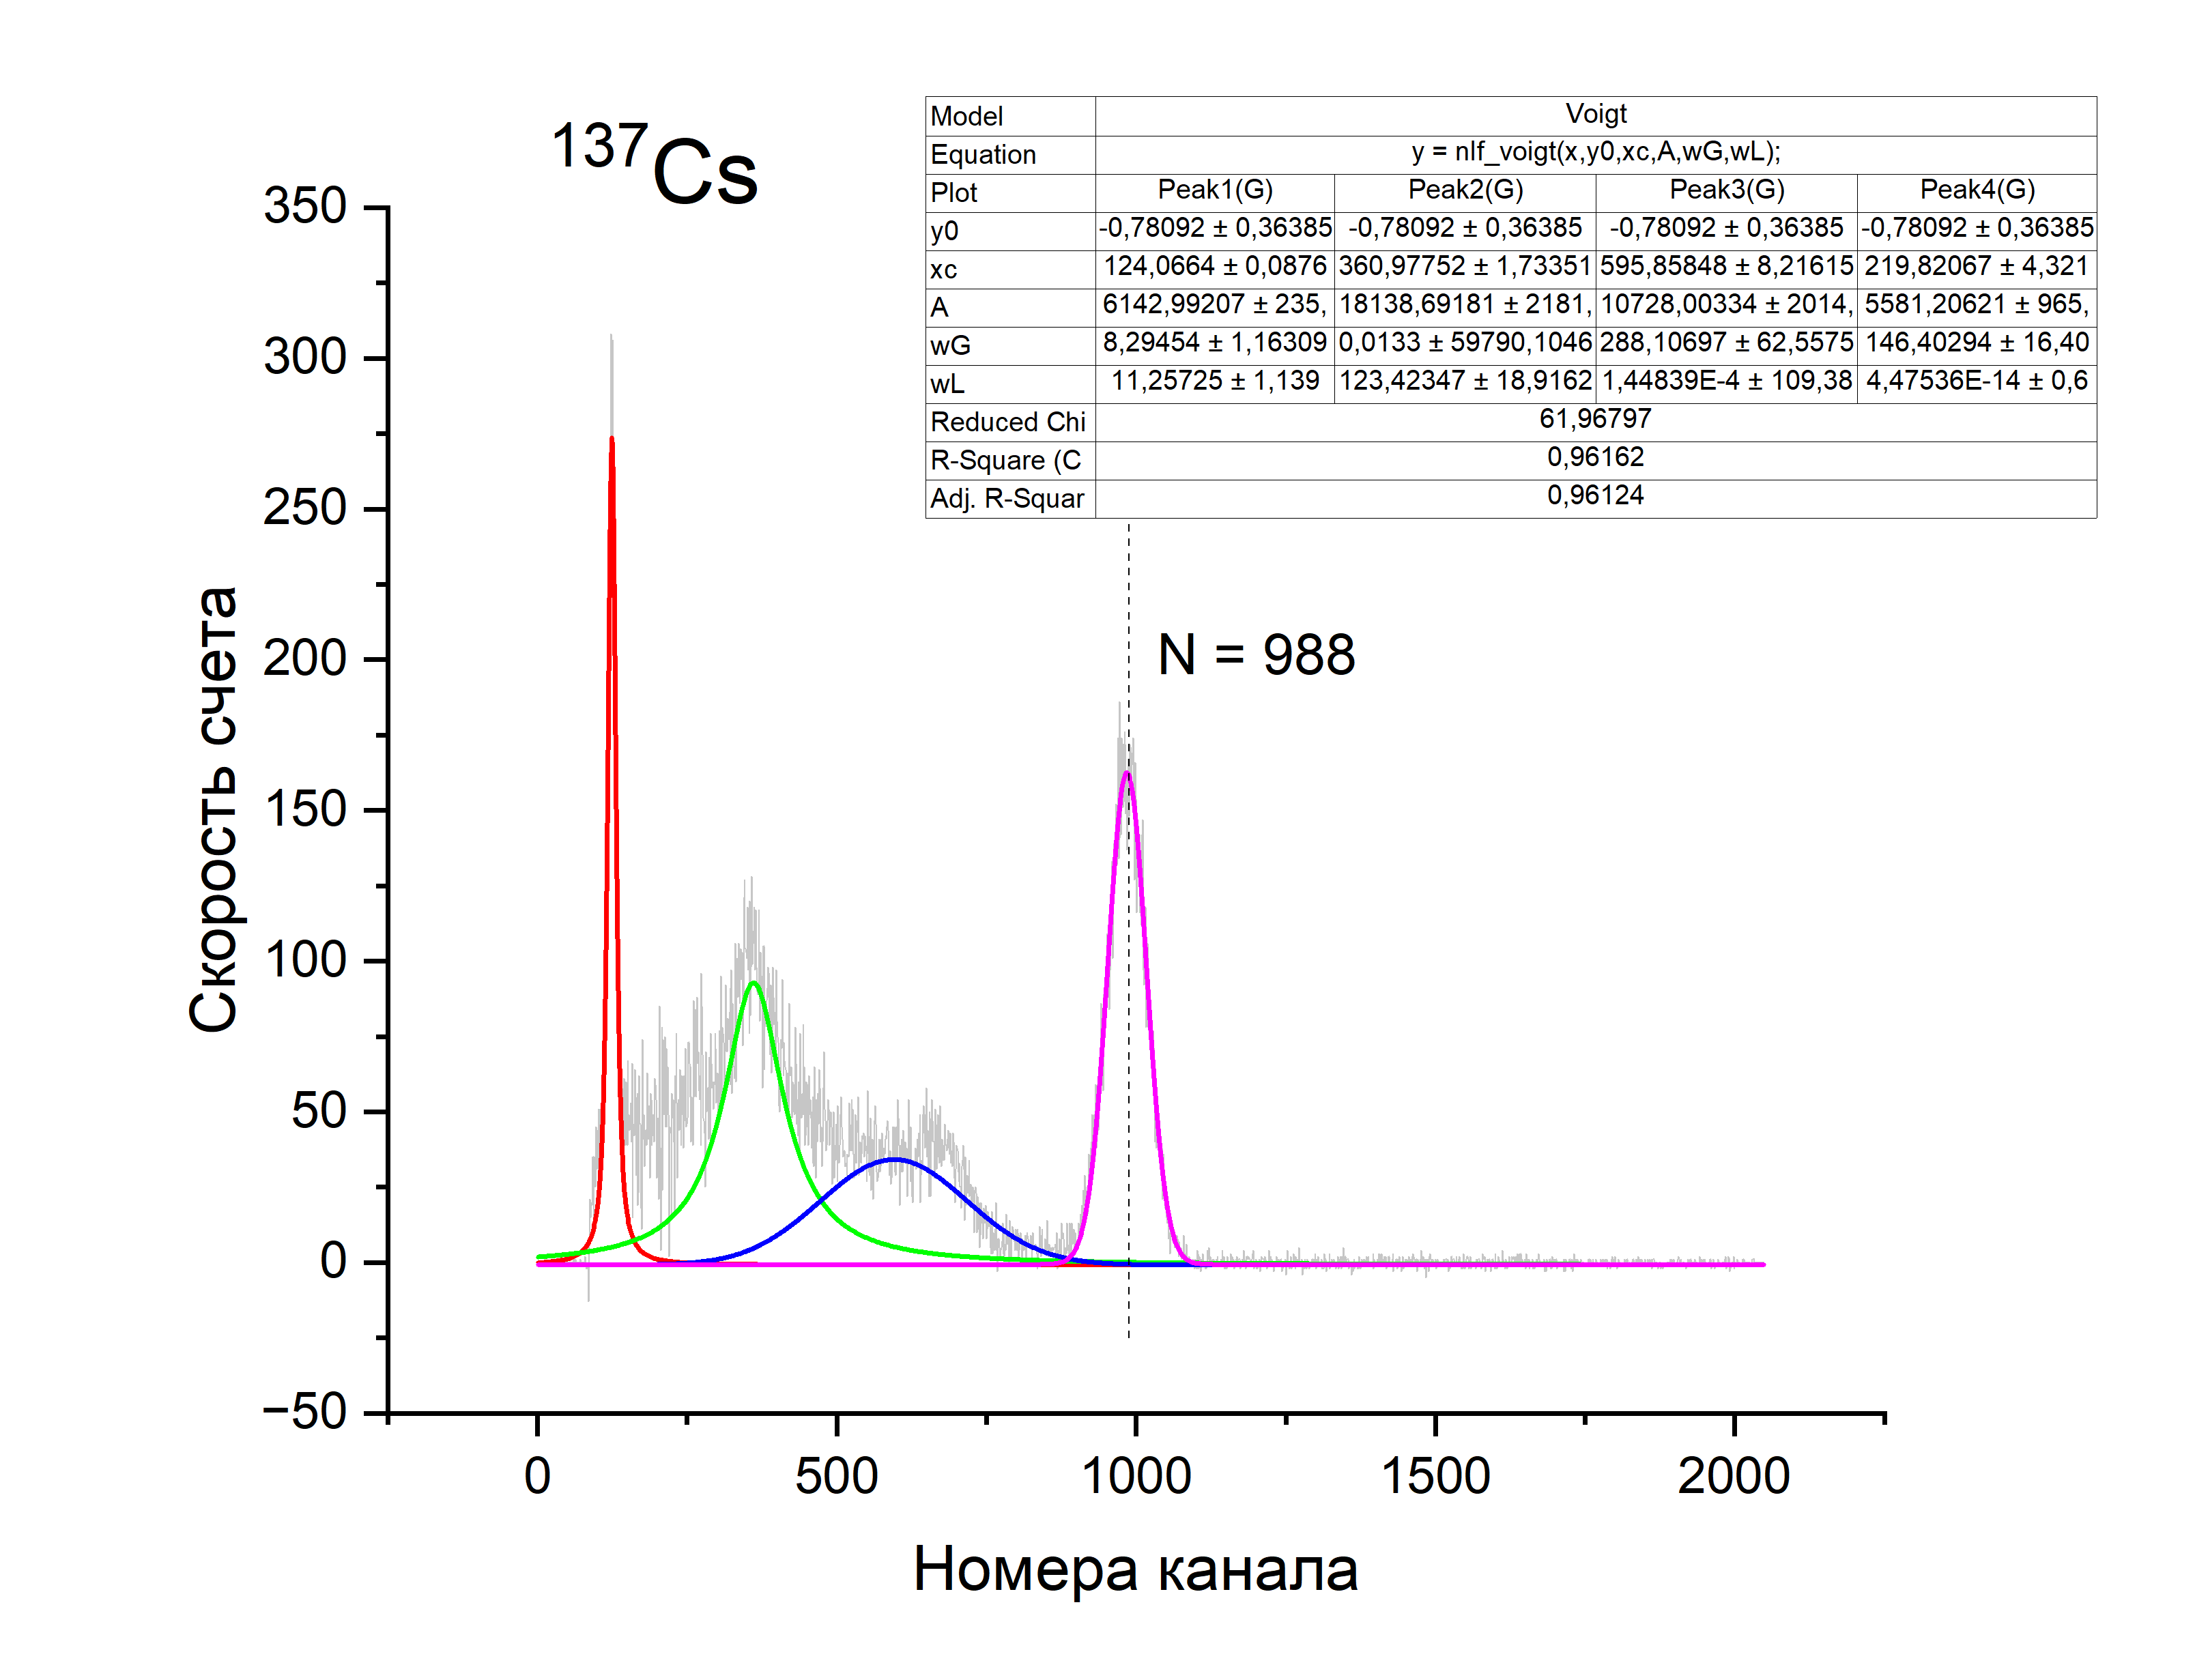
\includegraphics[scale=0.5]{cs.png}
    \caption{Спектр $^{137}Cs$}    
\end{figure}

\begin{figure}[h!]
    \centering
    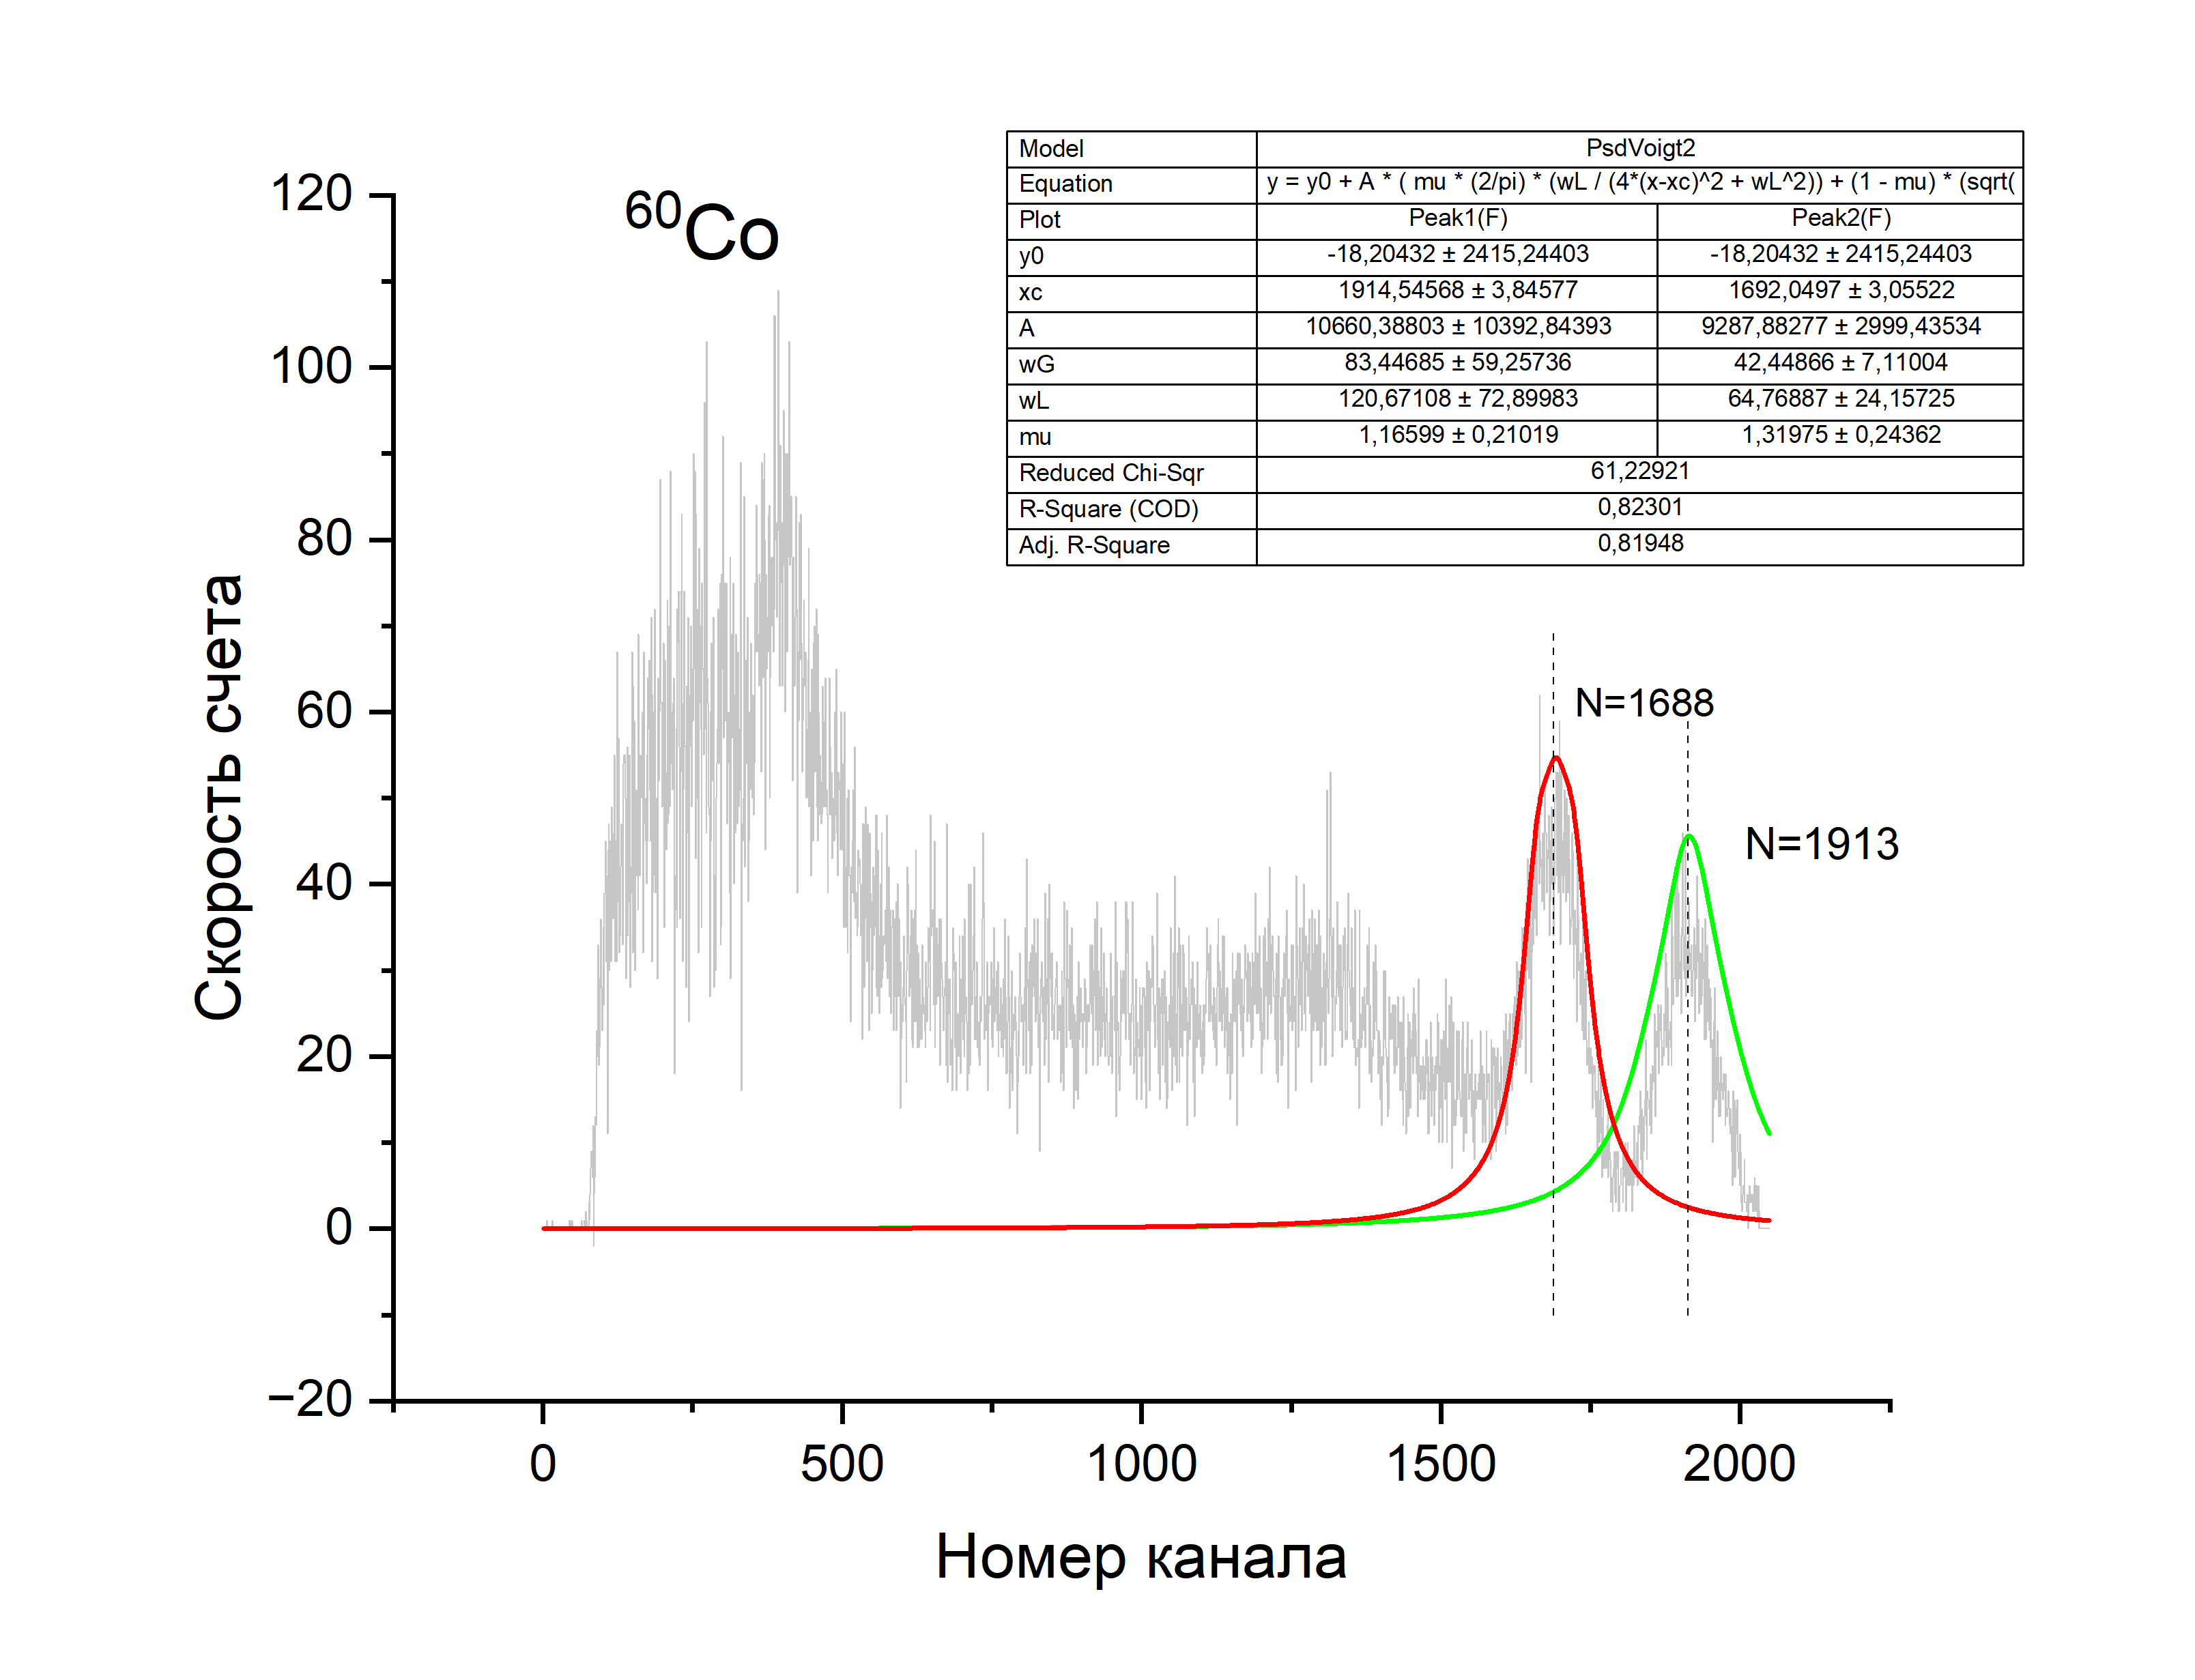
\includegraphics[scale=0.5]{co.png}
    \caption{Спектр $^{60}Co$}
\end{figure}


\begin{figure}[h!]
    \centering
    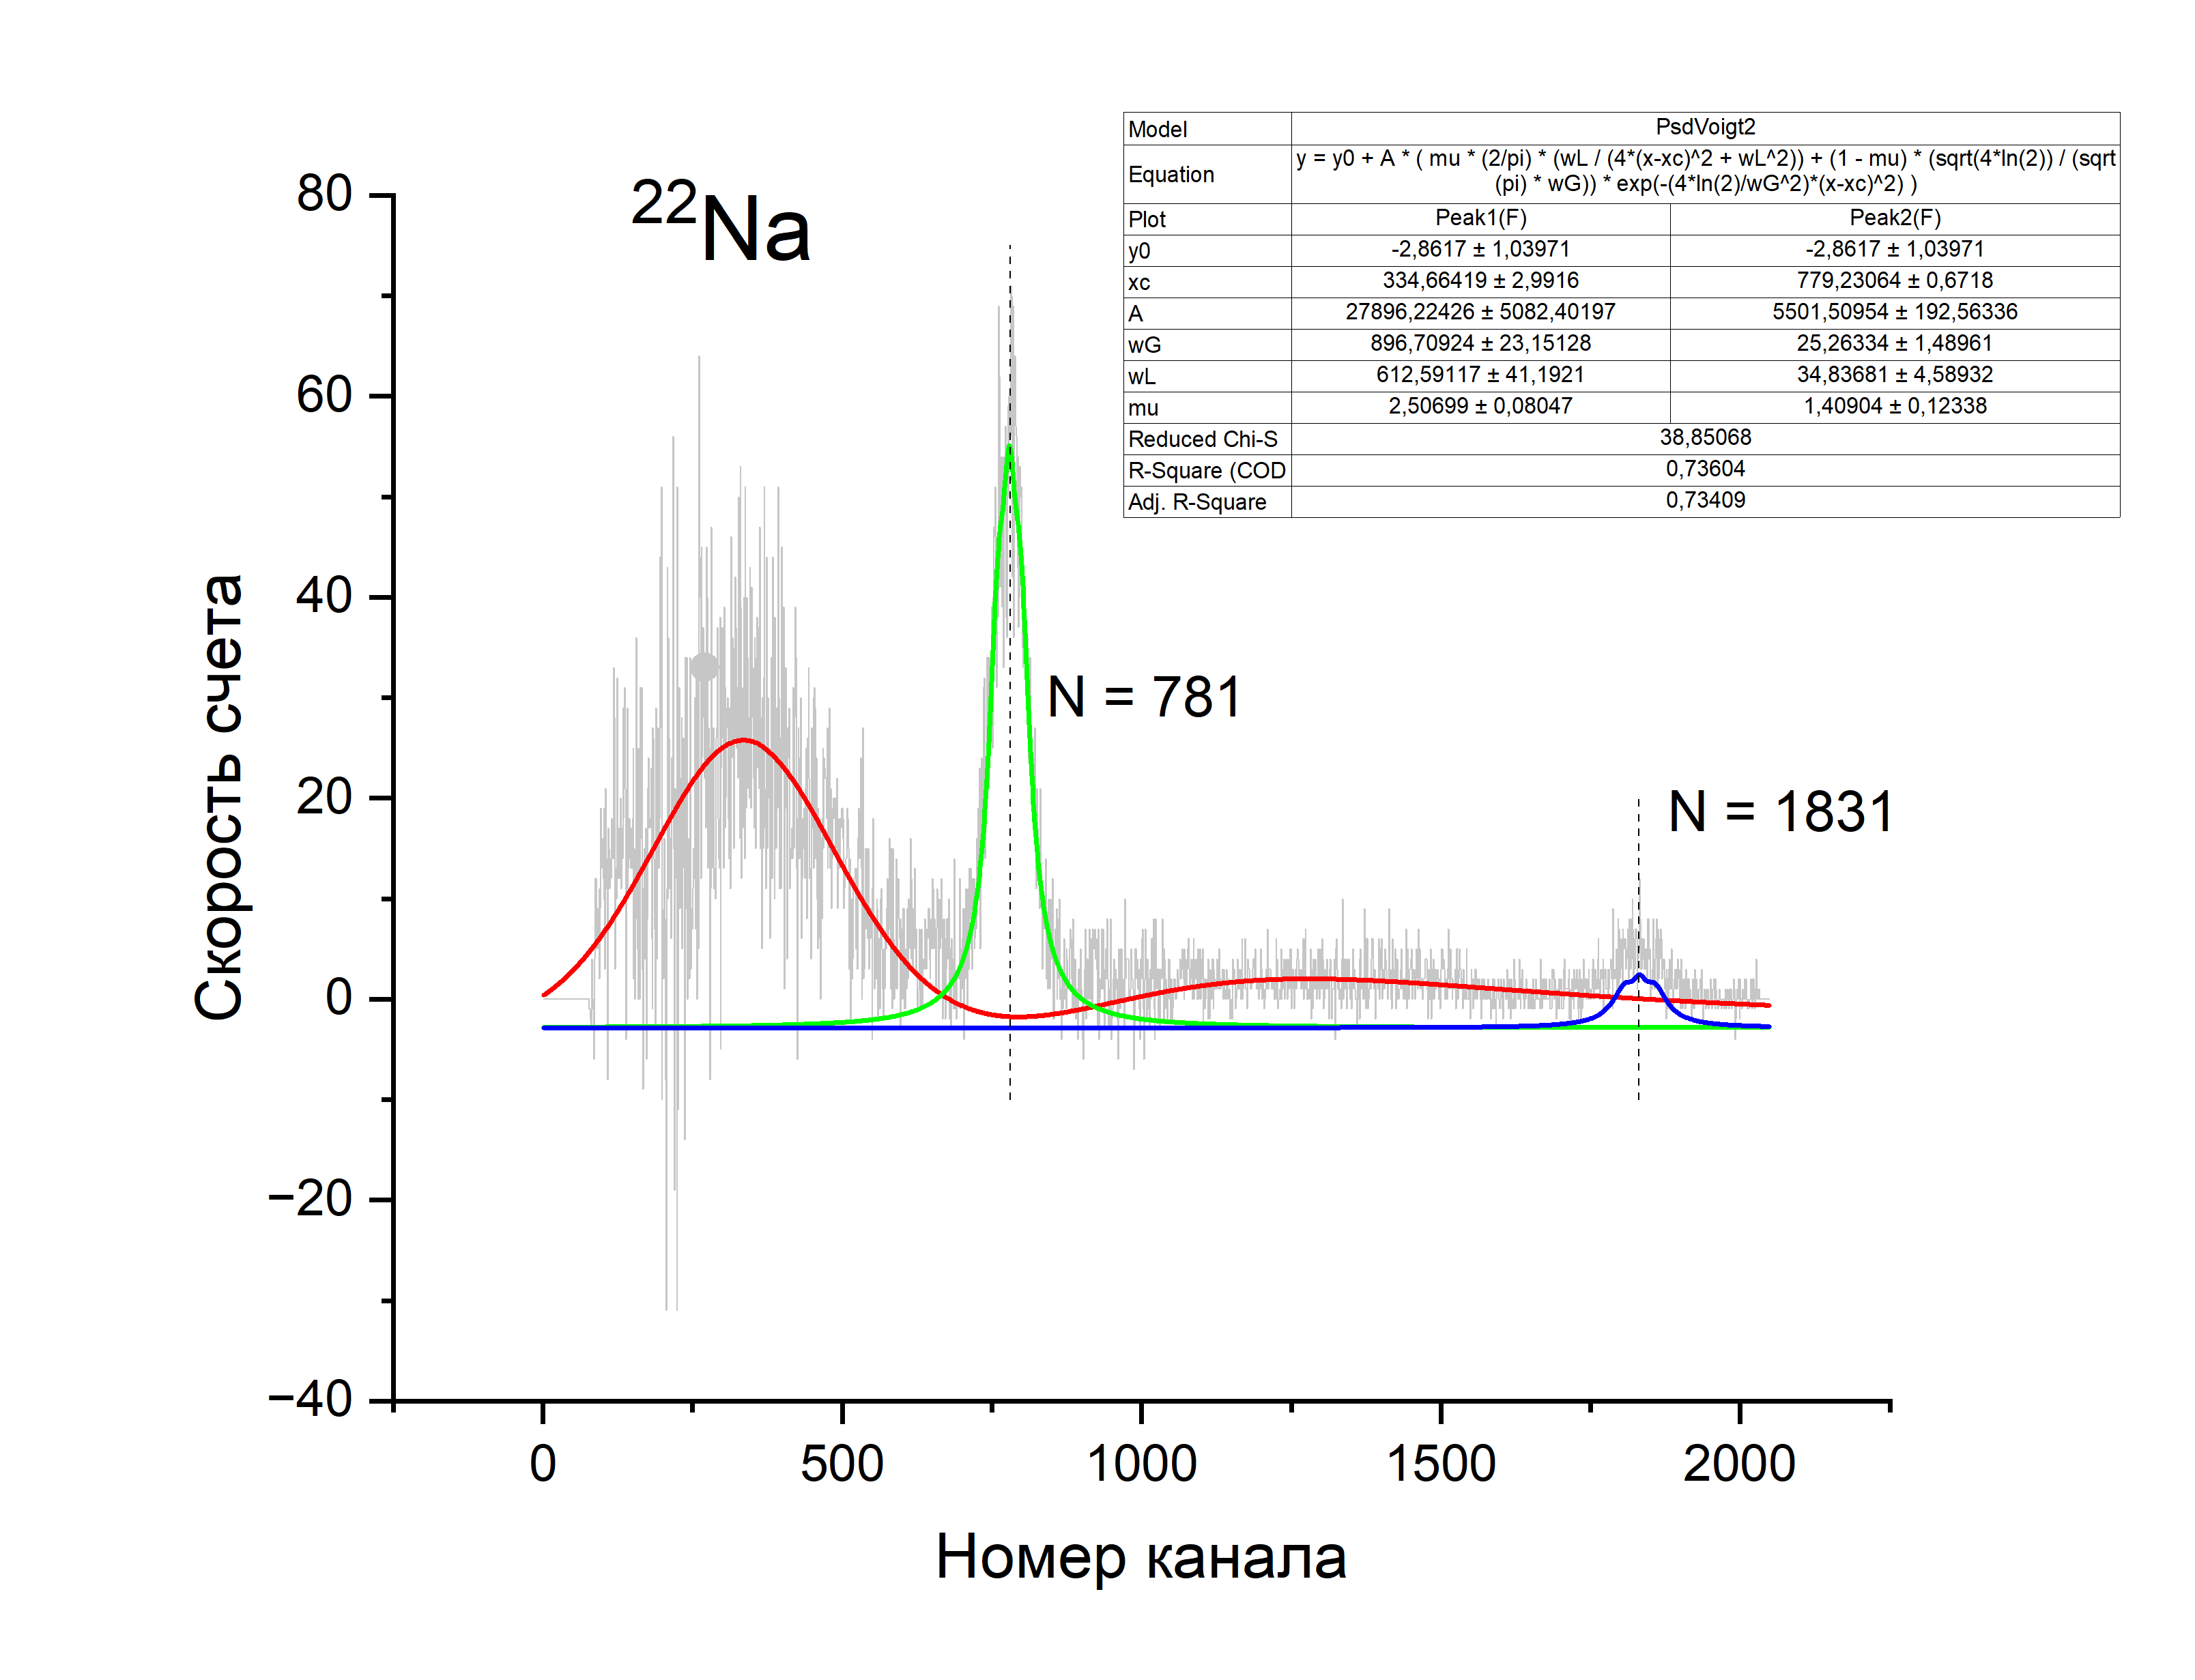
\includegraphics[scale=0.5]{na.png}
    \caption{Спектр $^{22}Na$}
\end{figure}

\begin{figure}[h!]
    \centering
    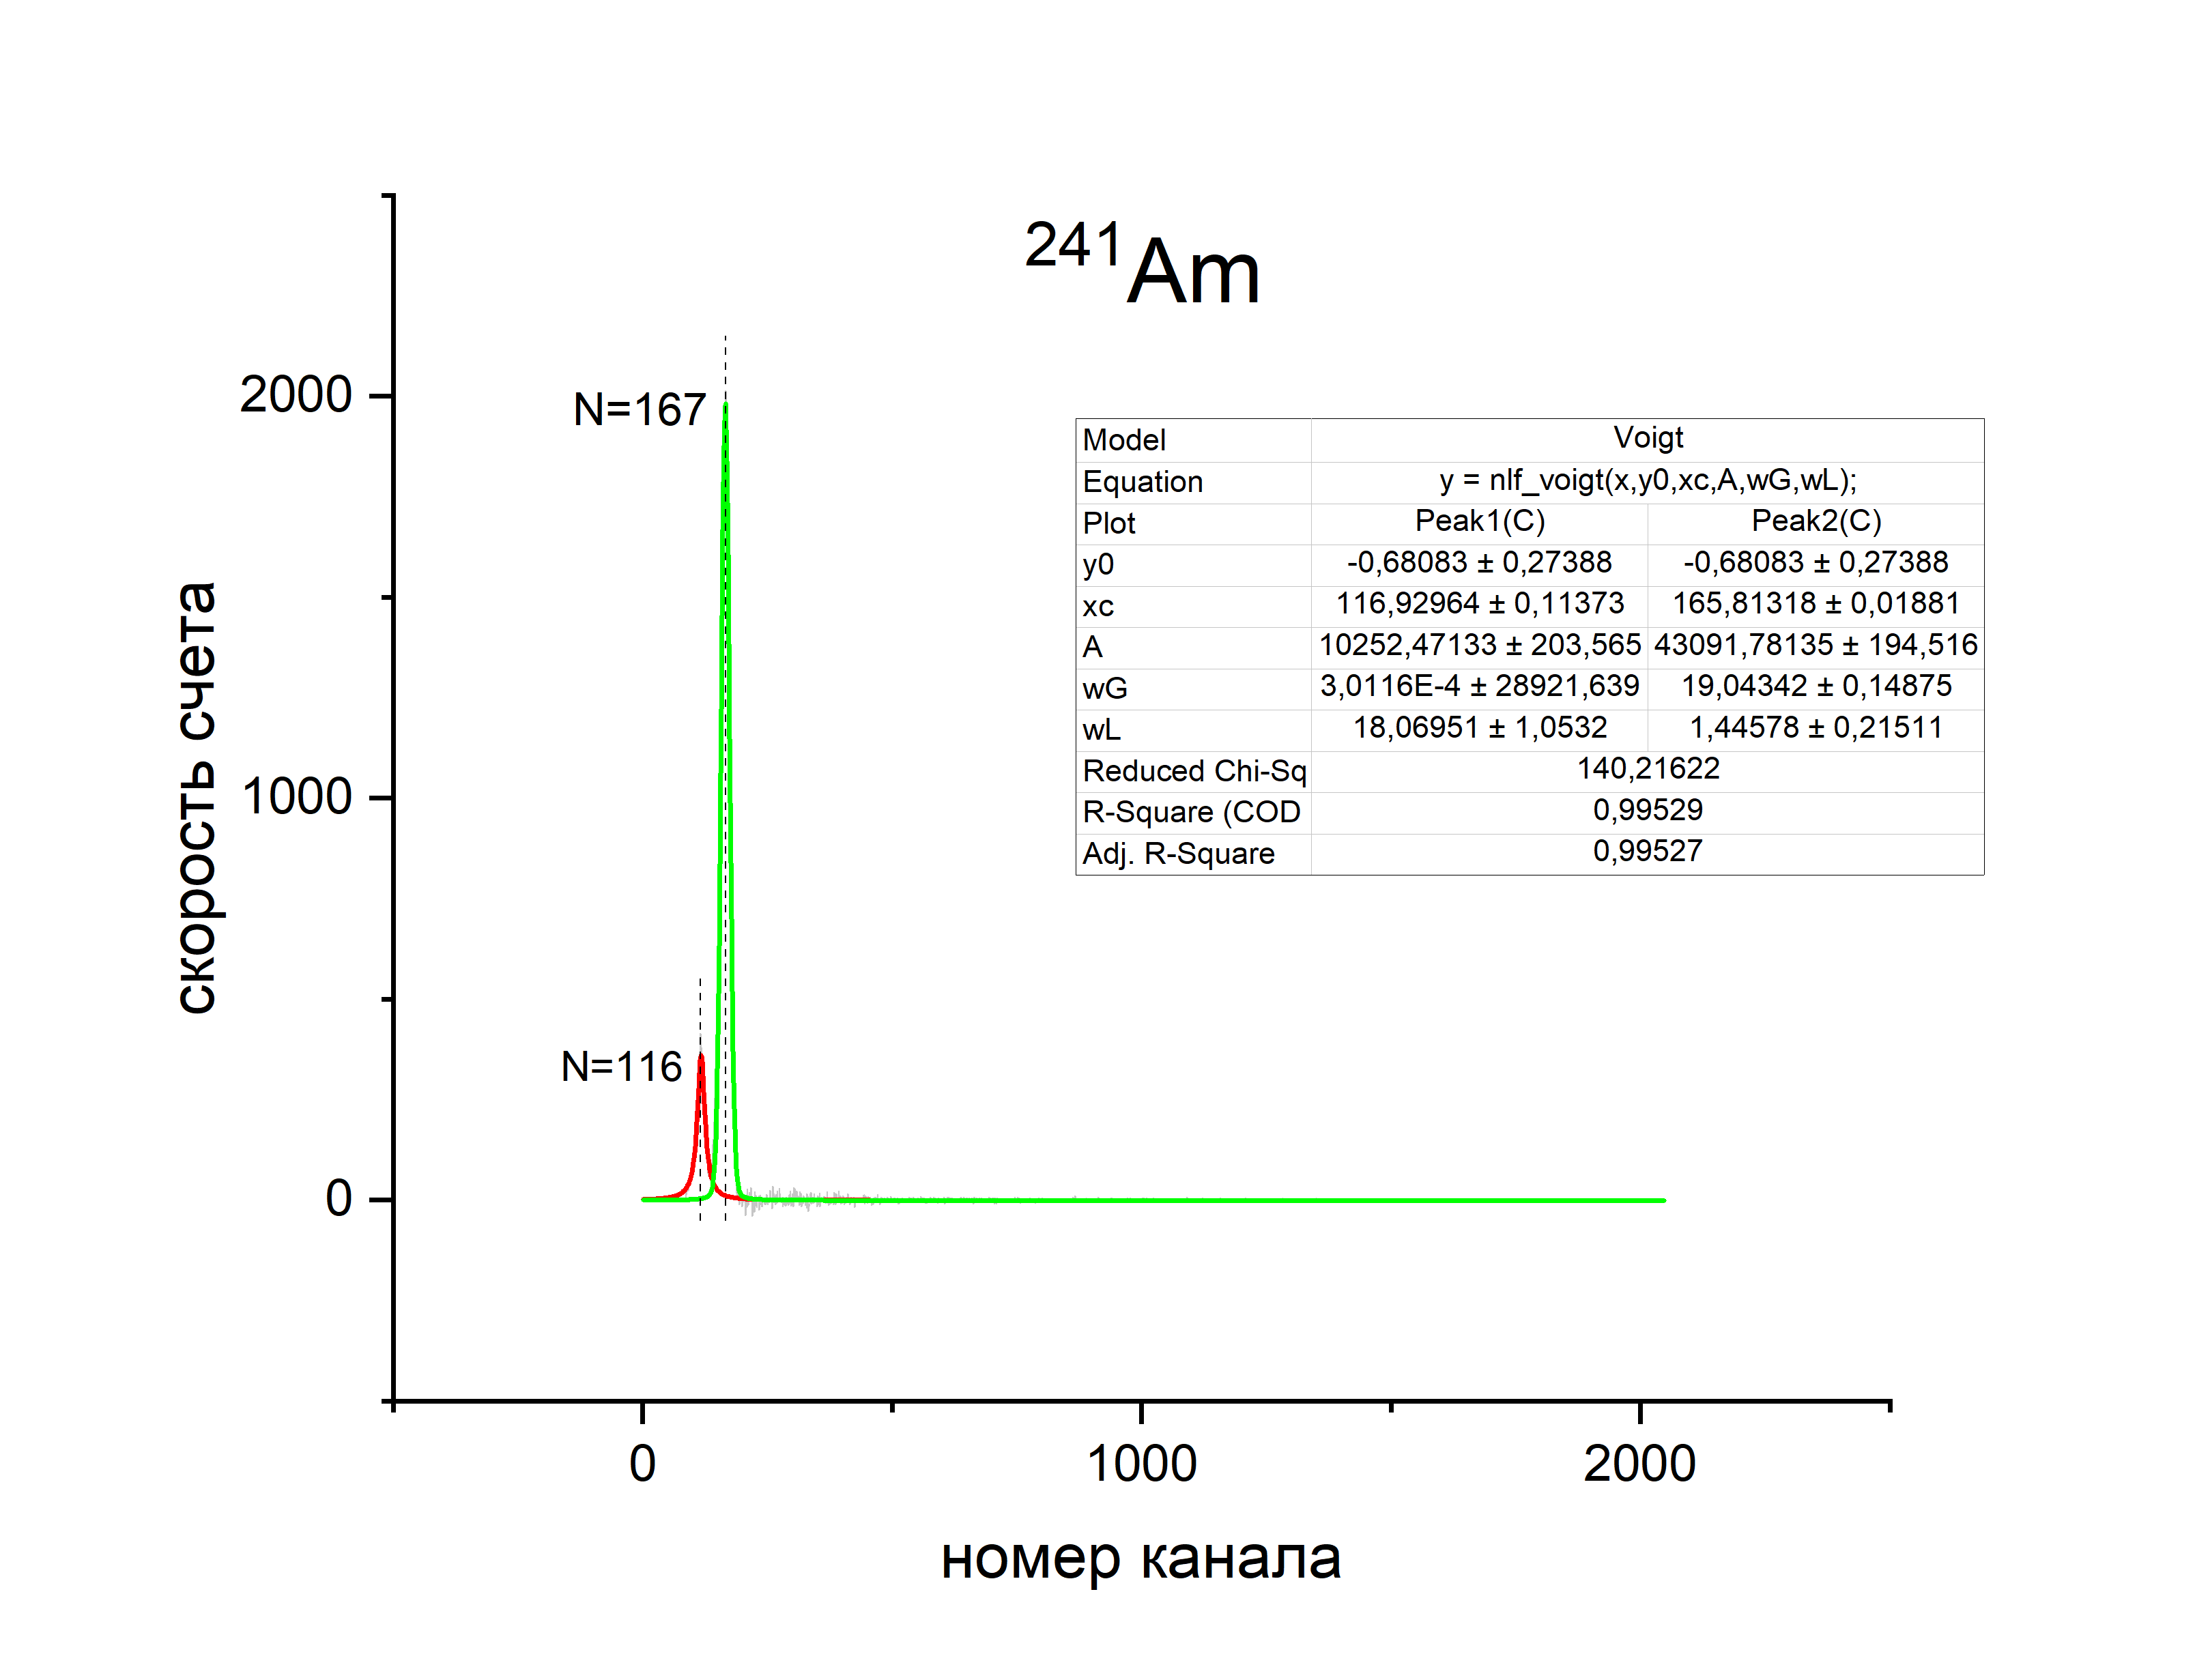
\includegraphics[scale=0.5]{am.png}
    \caption{Спектр $^{241}Am$}
\end{figure}


\begin{figure}[h!]
    \centering
    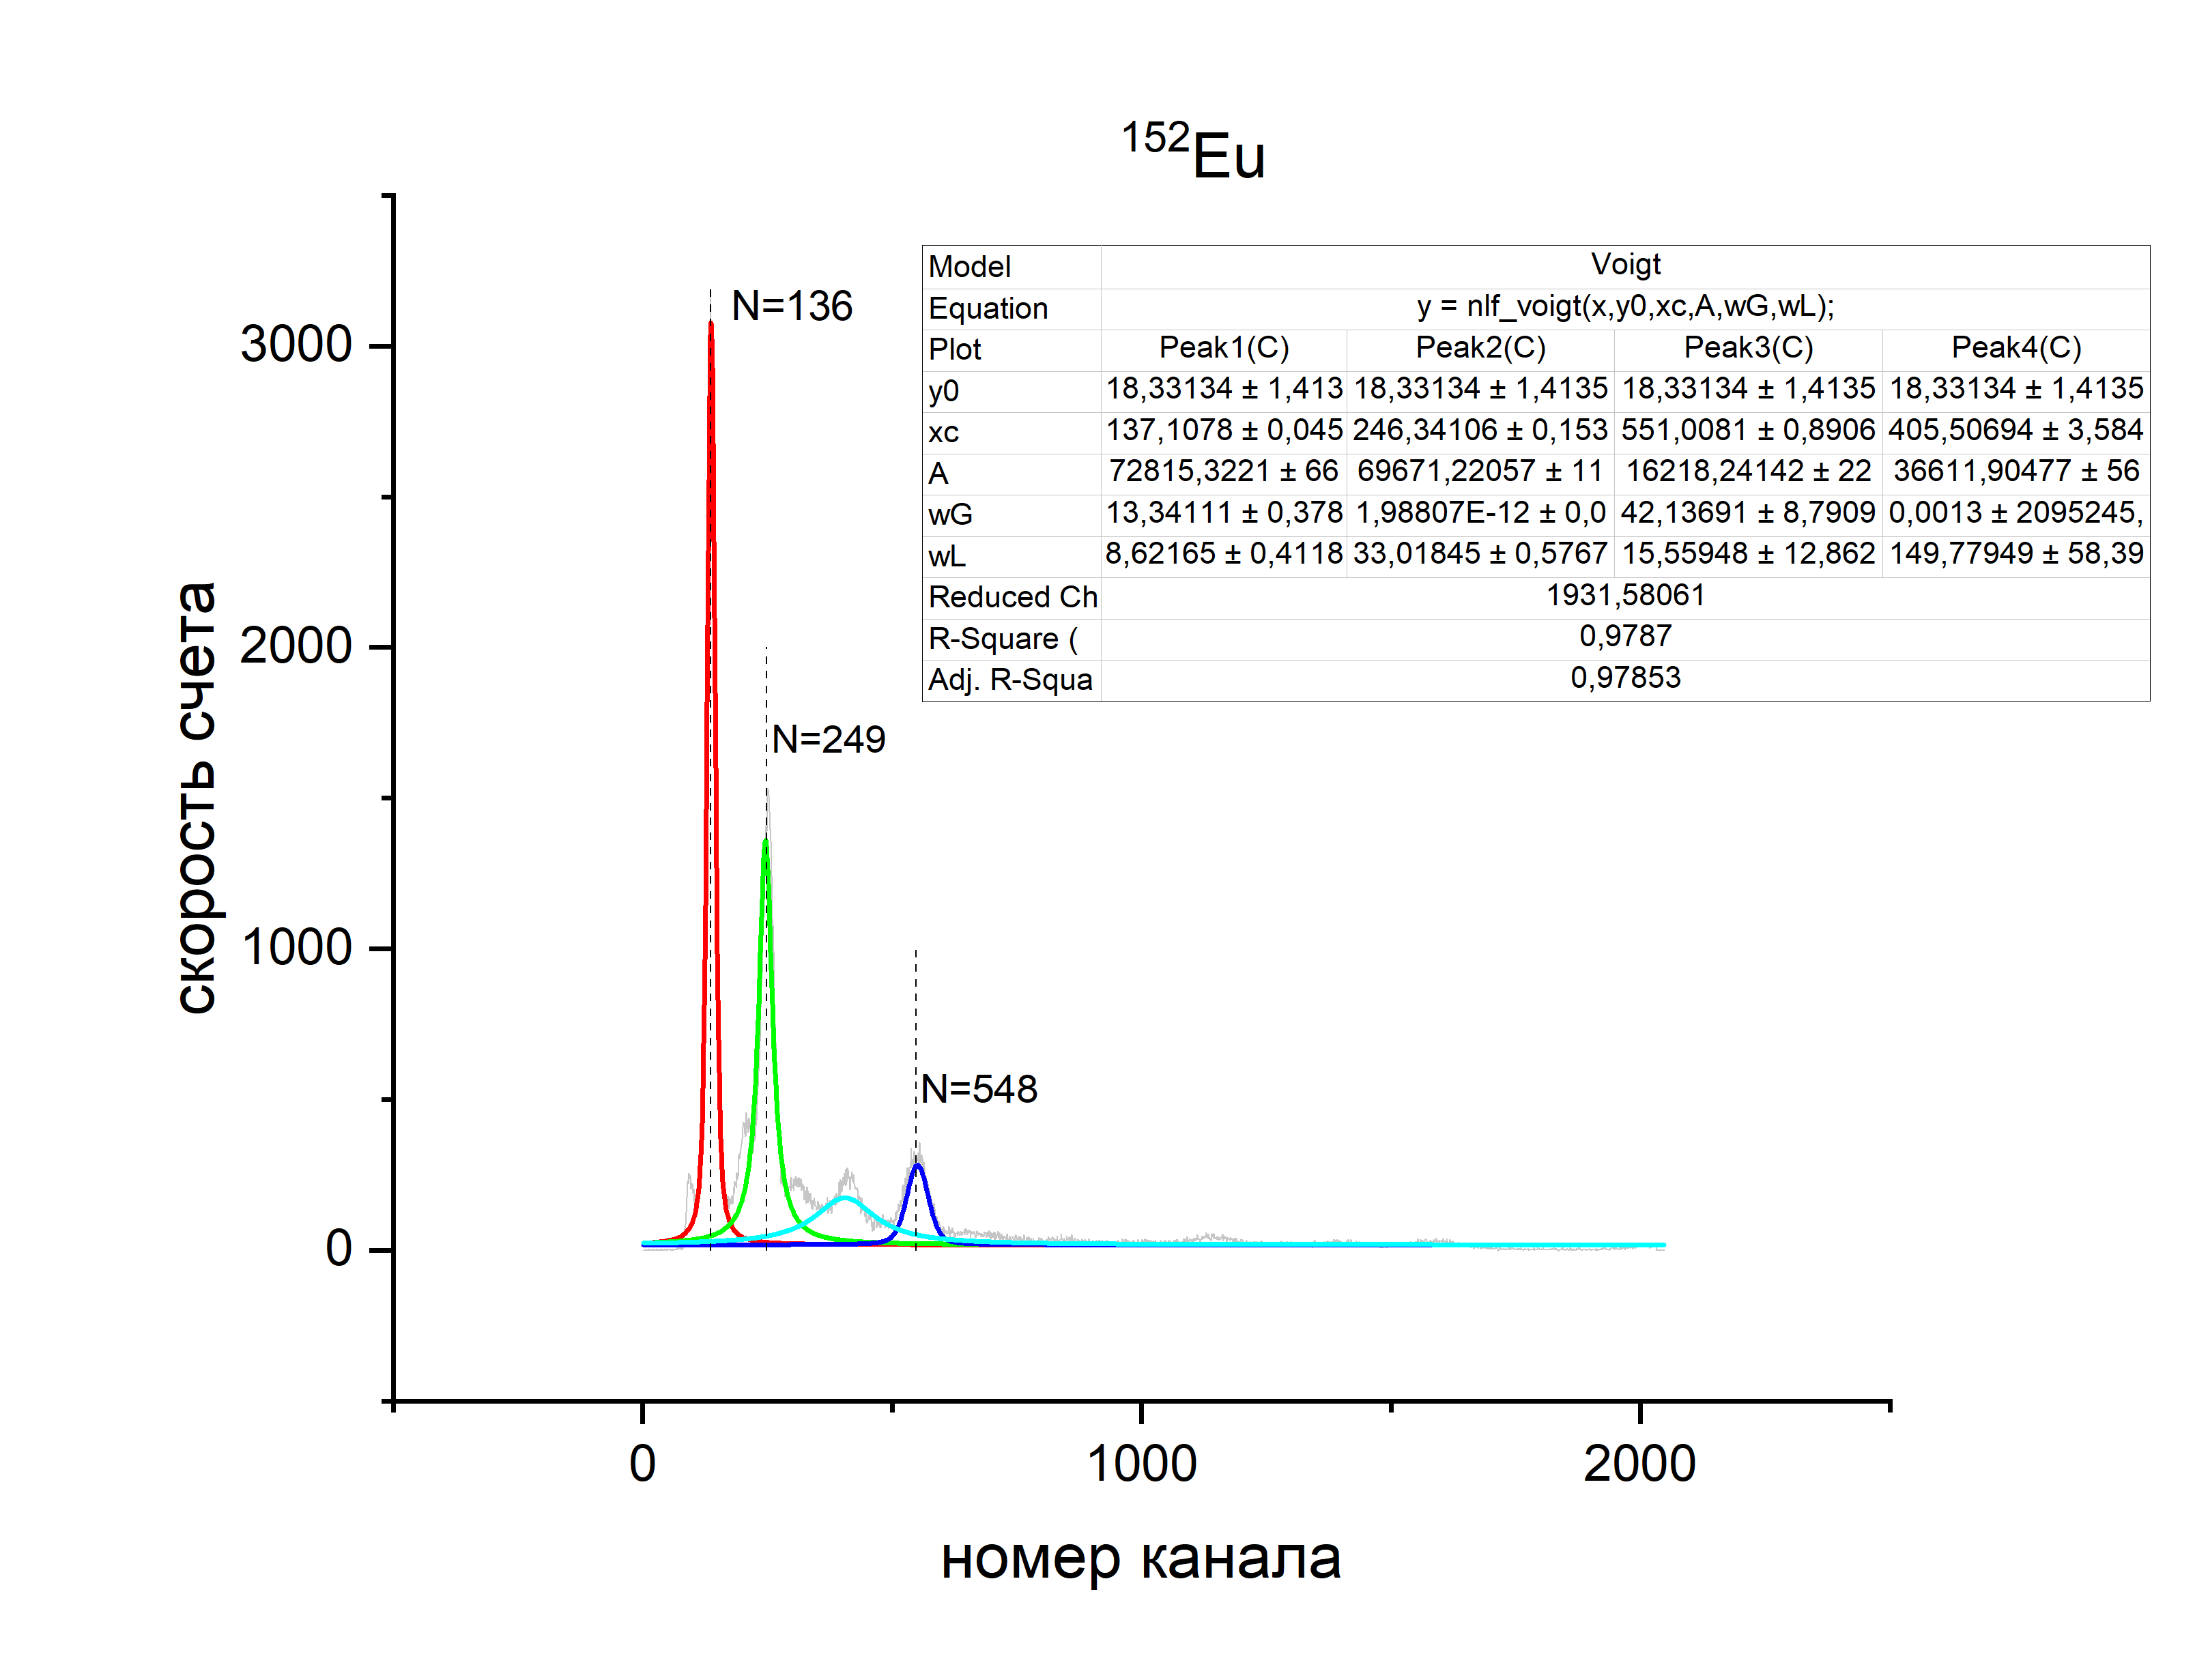
\includegraphics[scale=0.5]{eu.png}
    \caption{Спектр $^{152}Eu$}
\end{figure}


\end{document}